% ---------------------------------------------------------------------
% Para revisar sem as figuras, descomente a linha abaixo (as imagens
% viram caixas). Comente-a novamente na versão final.
% \PassOptionsToPackage{draft}{graphicx}
% ---------------------------------------------------------------------
\documentclass[11pt,a4paper,oneside]{book}
\usepackage[T1]{fontenc}
\usepackage[utf8]{inputenc}
\usepackage[brazilian]{babel}
\usepackage[margin=2.5cm]{geometry}
\usepackage{lmodern,microtype,amsmath,amssymb}
\usepackage{booktabs,tabularx,array}
\usepackage{float}
\usepackage{placeins}
\usepackage{graphicx}
\graphicspath{{figures/}{docs/figures/}}
\usepackage{tikz}
\usetikzlibrary{arrows.meta,positioning,shapes.geometric}
\usepackage{xurl}
\usepackage[hidelinks]{hyperref}
\hypersetup{
 pdftitle={Introdução aos enxames de drones},
 pdfauthor={João Leonardi da Silva Melo}
}
\usepackage{enumitem}
\setlength{\parindent}{1.2cm}
\setlength{\parskip}{0.3em}
\setlength{\emergencystretch}{2em}
\clubpenalty=10000
\widowpenalty=10000
\renewcommand{\topfraction}{0.9}
\renewcommand{\bottomfraction}{0.8}
\renewcommand{\textfraction}{0.1}
\renewcommand{\floatpagefraction}{0.75}
\setlength{\textfloatsep}{12pt plus 2pt minus 2pt}
\setlength{\intextsep}{10pt plus 2pt minus 2pt}
\setlist{itemsep=0.2em}
\setcounter{tocdepth}{1}
\numberwithin{equation}{chapter}
\addto\captionsbrazilian{%
 \renewcommand{\contentsname}{Sumário}%
 \renewcommand{\listfigurename}{Lista de figuras}%
 \renewcommand{\listtablename}{Lista de tabelas}%
 \renewcommand{\bibname}{Referências}%
}
\renewcommand{\arraystretch}{1.08}
\newcolumntype{Y}{>{\raggedright\arraybackslash}X}


\begin{document}

%======================================================================
\frontmatter
% Página de capa na proporção do JPEG (1250 x 1591), sem margens ou recorte.
% O grupo limita a mudança de tamanho à capa; as demais páginas continuam A4.
\begingroup
\setlength{\paperheight}{1.2728\paperwidth}
\pdfpageheight=\paperheight
\begin{titlepage}
\thispagestyle{empty}
\begin{tikzpicture}[remember picture,overlay]
\node at (current page.center) {
\includegraphics[width=\paperwidth,height=\paperheight,keepaspectratio]{capa.jpeg}};
\end{tikzpicture}
\null
\end{titlepage}
\endgroup

\begin{titlepage}
\centering
\vspace*{3.5cm}
{\Huge\bfseries Introdução aos\\[0.3em] enxames de drones\par}
\vspace{1.2cm}
{\Large Algoritmos, eletrônica, aviônica, simulação\\e plataformas de pesquisa\par}
\vspace{1.2cm}
{\Large João Leonardi da Silva Melo\par}
\vfill
% {\footnotesize Imagem da página anterior: capa de \emph{Science Robotics},\\
% v.~7, n.~66, maio de 2022 --- AAAS.\par}
\vspace{0.8cm}
{\large Outubro de 2026\par}
\vspace*{2cm}
\end{titlepage}

\chapter*{Prefácio}
\addcontentsline{toc}{chapter}{Prefácio}
O estudo de enxames de drones envolve dois problemas relacionados: o voo de cada aeronave e a coordenação do grupo. Compreender essa relação exige conhecimentos de controle, percepção, comunicação e planejamento. Este livro apresenta esses fundamentos e os relaciona às escolhas de software, eletrônica e plataformas utilizadas em projetos de pesquisa.

O texto apresenta os fundamentos de enxames de drones e relaciona a organização desses sistemas às escolhas de projeto e aos recursos disponíveis. As equações e os exemplos têm finalidade didática. Os estudos de caso ilustram soluções descritas na literatura e as condições em que foram avaliadas.

A exposição parte dos conceitos de enxame e da arquitetura funcional de uma aeronave, apresentados nos Capítulos~\ref{cap:intro} e~\ref{cap:arq}. Os Capítulos~\ref{cap:alg} a~\ref{cap:eletr} desenvolvem os fundamentos de algoritmos, comunicação, eletrônica e aviônica. O Capítulo~\ref{cap:sim} aborda a simulação e seus limites, e o Capítulo~\ref{cap:casos} examina quatro estudos de caso. Por fim, o Capítulo~\ref{cap:plat} reúne critérios para selecionar plataformas e identificar as competências necessárias à integração. O Apêndice~\ref{ap:glossario} apresenta o glossário de siglas, e o Apêndice~\ref{ap:notacao} reúne a notação matemática.

\tableofcontents
\listoffigures
\listoftables

%======================================================================
\mainmatter

%######################################################################
\chapter{Introdução}\label{cap:intro}
\section{Drones na pesquisa científica}\label{sec:drones-pesquisa}
Um drone é uma aeronave não tripulada que pode receber comandos de um operador ou executar funções de voo por meio de sistemas embarcados. O uso do termo não implica autonomia: estabilizar a atitude, seguir uma rota e perceber obstáculos são funções diferentes. Uma aeronave pode executar algumas delas automaticamente e ainda depender de decisões do operador.

Na pesquisa científica, o drone pode ser tanto o sistema investigado quanto uma plataforma para transportar instrumentos. Ao desenvolver um sensor, por exemplo, o interesse pode estar na qualidade das medições durante o voo. Ao investigar um novo algoritmo de controle, o objeto passa a ser a resposta da aeronave aos comandos. Em estudos de percepção e navegação, analisam-se formas de estimar a posição, interpretar imagens ou escolher trajetórias. Essas pesquisas podem utilizar uma única aeronave e exigem recursos diferentes de hardware e software~\cite{controle,companion,px4payloads}.

A escolha da plataforma acompanha essa diferença de objetivos. Uma aeronave integrada pode fornecer câmera e funções de voo prontas para aquisição de dados. Uma montagem própria permite selecionar sensores, alimentação e processamento, além de modificar o software quando a pilha de voo utilizada oferece esse acesso. A pilha de voo é o conjunto de módulos de software responsáveis por funções como estimação, controle e gerenciamento do voo. Estruturas como DJI F450 e HolyBRO X500 são exemplos de plataformas de integração discutidas neste livro; sua utilidade depende dos equipamentos e das interfaces exigidos pela pesquisa. A relação entre essas escolhas, as áreas de investigação e os conhecimentos necessários é desenvolvida no Capítulo~\ref{cap:plat}.

Quando a tarefa envolve várias aeronaves, é necessário coordenar seus movimentos, distribuir tarefas e compartilhar informações. O estudo de enxames combina, portanto, controle de voo, sensoriamento e navegação com mecanismos de comunicação e coordenação entre veículos.

\section{O que é um enxame de drones}
Neste texto, um enxame de drones é um conjunto de aeronaves cujas ações são coordenadas para executar uma tarefa coletiva, como manter uma formação ou explorar um ambiente. O número de aeronaves, isoladamente, não descreve o grau de autonomia: é necessário identificar quais decisões são calculadas em cada veículo e quais dependem de infraestrutura externa~\cite{survey}.

O termo é usado com sentidos diferentes. Em sentido estrito, associa-se à robótica de enxame: muitos agentes relativamente simples, que interagem por regras locais e não dependem de um controle central. Em sentido amplo, designa qualquer grupo coordenado de aeronaves, inclusive aquele em que uma estação central fornece posições ou comandos. Este livro adota o sentido amplo para discutir sistemas centralizados e descentralizados e identifica, em cada exemplo, onde as decisões são calculadas.

A navegação de um enxame combina problemas de escalas distintas. Cada aeronave precisa estimar seu estado e acompanhar comandos de movimento. O grupo precisa compatibilizar esses movimentos com obstáculos, outros veículos e objetivos da missão. Por isso, um algoritmo de formação não substitui o controlador que estabiliza a aeronave, e um controlador de atitude não resolve a coordenação do grupo. Essa distinção organiza a apresentação dos algoritmos e dos estudos de caso.

\section{Motivações e aplicações}
% O interesse em usar várias aeronaves, em vez de uma única, decorre de algumas propriedades potenciais do grupo: a cobertura paralela de uma área extensa; a redundância, pois a falha de um agente não necessariamente encerra a missão; a possibilidade de usar veículos pequenos e de menor custo individual; e a execução simultânea de tarefas em pontos distintos. O ganho depende dos recursos exigidos pela coordenação, pela comunicação e pela logística.
O uso de várias aeronaves pode permitir a cobertura paralela de uma área e a execução simultânea de tarefas em pontos distintos. A coordenação também pode oferecer redundância, quando os demais veículos conseguem assumir as tarefas de uma aeronave que falhou. Esses benefícios dependem dos recursos exigidos pela comunicação, pela coordenação e pela logística de operação.

% Entre as aplicações frequentemente mencionadas estão o mapeamento e a inspeção de estruturas, a busca em áreas extensas, o monitoramento ambiental e agrícola, as exibições coreografadas e a própria pesquisa em robótica. A lista é ilustrativa; este livro não avalia a maturidade tecnológica ou comercial de cada aplicação, e as condições de cada uma (ambiente, regulação, tolerância a falhas) alteram os requisitos do sistema.
As aplicações de enxames de drones incluem mapeamento, inspeção de estruturas, busca em áreas extensas, monitoramento ambiental e agrícola, exibições coreografadas e pesquisa em robótica. Cada aplicação exige diferentes condições de operação, recursos de coordenação e tolerância a falhas. Os exemplos situam os possíveis usos dos enxames; este texto não avalia sua maturidade tecnológica ou comercial.

\section{Restrições de projeto e operação}
O projeto de um enxame precisa considerar restrições de sensoriamento, comunicação e computação, discutidas na revisão sobre microveículos aéreos~\cite{survey}, além de requisitos de massa, energia, segurança e reprodutibilidade:
\begin{itemize}
\item \emph{massa, energia e tempo de voo}: sensores e computadores acrescentam massa e consumo e podem reduzir o tempo de voo;
\item \emph{sensoriamento e localização}: sem infraestrutura externa, o sistema precisa estimar posição e perceber obstáculos com sensores embarcados;
\item \emph{comunicação}: enlaces têm alcance, atraso e capacidade limitados, e podem falhar;
\item \emph{computação}: o cálculo precisa terminar dentro do tempo disponível em processadores de bordo limitados;
\item \emph{segurança operacional}: um defeito ou uma falha de coordenação pode afetar vários veículos ao mesmo tempo;
\item \emph{reprodutibilidade}: reproduzir resultados exige documentar montagem, calibração, software e condições do ambiente.
\end{itemize}

\section{Critérios de classificação de enxames}\label{sec:eixos}
O número de drones não é suficiente para caracterizar um enxame. Quatro critérios ajudam a descrever sua organização e suas condições de operação:
\begin{enumerate}
\item \emph{Distribuição das decisões}: quais funções são executadas em uma estação central, em cada aeronave ou de forma compartilhada.
\item \emph{Fonte de localização}: quais informações provêm de infraestrutura externa, como captura de movimento, e quais são obtidas por sensores embarcados.
\item \emph{Ambiente de operação}: se o espaço é interno ou externo, quais obstáculos estão presentes e a quais perturbações os veículos estão sujeitos.
\item \emph{Forma de avaliação}: se os resultados foram obtidos em simulação, em voos reais ou em ambos, e sob quais condições.
\end{enumerate}
A Tabela~\ref{tab:eixos} caracteriza os quatro estudos de caso do Capítulo~\ref{cap:casos} segundo esses critérios. Essa organização tem finalidade didática e foi elaborada a partir das descrições dos trabalhos.

\begin{table}[htbp]
\centering\small
\caption{Classificação dos estudos de caso do Capítulo~\ref{cap:casos} segundo os critérios da Seção~\ref{sec:eixos}.}
\label{tab:eixos}
\begin{tabularx}{\textwidth}{@{}>{\raggedright\arraybackslash}p{2.4cm}YYYY@{}}
\toprule
Estudo & Decisões & Localização & Ambiente & Avaliação \\
\midrule
Crazyswarm~\cite{crazyswarm} & Estação fornece posições; controle a bordo & Captura de movimento (externa) & Interno & Voo real, nanoquadricópteros \\
Floresta de bambu~\cite{wildpaper} & Percepção, estimação e planejamento a bordo & Embarcada & Externo, com obstáculos & Voo real \\
SwarmLab~\cite{swarmlab} & Regras do algoritmo simulado & Idealizada pelo modelo & Simulado & Simulação \\
SGBA~\cite{mcguire} & Comportamentos reativos a bordo & Sensores de distância e fluxo óptico & Ambiente desconhecido & Voo real, microcontrolador \\
\bottomrule
\end{tabularx}
\end{table}

\section{Notação}
Os símbolos utilizados nas equações estão reunidos na Tabela~\ref{tab:notacao}, no Apêndice~\ref{ap:notacao}. Quando um símbolo é usado com outro sentido, isso é indicado no texto.

\section{Escopo e limitações}\label{sec:escopo}
A seleção bibliográfica é introdutória: não resulta de busca sistemática e não classifica algoritmos ou plataformas quantitativamente. As equações são didáticas e não reproduzem implementações publicadas. As recomendações de componentes e de plataformas são critérios de projeto derivados da documentação consultada, e não configurações validadas experimentalmente. As comparações organizam requisitos e interfaces; não estabelecem diferenças medidas de custo ou desempenho. As figuras reproduzidas de outros autores registram as condições dos respectivos estudos e não implicam desempenho equivalente em outras condições. Nenhum preço foi levantado e nenhuma plataforma foi ensaiada para este texto. A documentação técnica citada (em especial a do PX4) muda com o tempo; as referências indicam a versão consultada.

%######################################################################
\chapter{Arquitetura funcional de um drone em enxame}\label{cap:arq}
\section{Camadas funcionais}
A Figura~\ref{fig:camadas} apresenta uma organização funcional para interpretar um sistema autônomo. O planejamento recebe objetivos, mapas e estados estimados e produz referências de movimento. O controle acompanha essas referências, enquanto a estimação atualiza o estado utilizado pelos demais módulos. A comunicação fornece informações sobre outros agentes quando o algoritmo exige essa troca.

\begin{figure}[htbp]
\centering
\begin{tikzpicture}[node distance=7mm,box/.style={draw,rounded corners,align=center,text width=10cm,minimum height=9mm,font=\small},>=Latex]
\node[box] (missao) {Missão e coordenação do enxame};
\node[box,below=of missao] (plan) {Planejamento de trajetórias e prevenção de colisões};
\node[box,below=of plan] (cont) {Controle de posição, velocidade e atitude};
\node[box,below=of cont] (act) {Alocação de controle, motores e movimento da aeronave};
\node[box,below=of act] (est) {Sensores e estimação de estado};
\draw[->] (missao)--(plan);
\draw[->] (plan)--(cont);
\draw[->] (cont)--(act);
\draw[->] (act)--(est);
\draw[->] (est.west)--++(-7mm,0)|-(cont.west);
\draw[->] (est.east)--++(7mm,0)|-(plan.east);
\end{tikzpicture}
\caption[Organização funcional do voo autônomo em enxame]{Organização funcional de um drone autônomo integrado a um enxame. As setas de retorno representam o uso do estado estimado no planejamento e no controle. Esquema conceitual elaborado para este livro.}
\label{fig:camadas}
\end{figure}

Cada bloco da Figura~\ref{fig:camadas} responde a uma pergunta diferente. A camada de missão decide \emph{o que} cada aeronave faz. O planejamento decide \emph{por onde} e \emph{quando} se move. O controle decide \emph{quais comandos} aplicar para seguir o movimento planejado. A estimação responde a \emph{onde a aeronave está e com que velocidade se move}. A Tabela~\ref{tab:camadas} associa cada camada aos algoritmos e capítulos correspondentes.

\begin{table}[htbp]
\centering\small
\caption{Camadas funcionais, exemplos de algoritmos e capítulos em que são tratados.}
\label{tab:camadas}
\begin{tabularx}{\textwidth}{@{}>{\raggedright\arraybackslash}p{3.6cm}YY@{}}
\toprule
Camada & Exemplos tratados & Capítulo \\
\midrule
Missão e coordenação & Alocação de tarefas (CBBA), consenso, líder--seguidor, Boids & \ref{cap:alg} \\
Planejamento e colisões & ORCA, planejamento de trajetórias (EGO-Swarm), MPC & \ref{cap:alg} \\
Controle & Cascata e PID, alocação de controle & \ref{cap:alg} \\
Estimação e localização & EKF, localização relativa (UWB, visão) & \ref{cap:alg}, \ref{cap:com} \\
Comunicação & Topologias, enlaces, perda de comunicação & \ref{cap:com} \\
Hardware e integração & Controladora, computador complementar, sensores, propulsão & \ref{cap:eletr} \\
\bottomrule
\end{tabularx}
\end{table}

\section{Escalas de tempo}
As camadas operam em taxas e com requisitos de latência diferentes. O controle de atitude exige atualização rápida, da ordem de centenas de hertz em plataformas típicas; o ciclo embarcado do Crazyswarm, por exemplo, operou a 500~Hz nas condições descritas no artigo~\cite{crazyswarm}. O planejamento de trajetórias costuma operar a taxas bem menores, e a alocação de tarefas, a taxas menores ainda. Essa diferença de escalas orienta a divisão de funções entre a controladora de voo, que executa as tarefas mais rápidas e críticas, e o computador complementar, que executa as mais pesadas e menos frequentes (Capítulo~\ref{cap:eletr}).

Uma consequência prática é que o atraso introduzido em uma camada afeta as demais. Um planejador lento entrega referências desatualizadas ao controle; uma estimação com atraso faz o controle agir sobre um estado que já mudou. Por isso, o projeto de um enxame deve explicitar, para cada interface da Figura~\ref{fig:camadas}, a frequência e a latência esperadas.

\section{Distribuição das decisões}
A arquitetura funcional não determina onde cada camada é executada. Em uma arquitetura \emph{centralizada}, uma estação calcula trajetórias ou comandos de todos os agentes e os transmite. Isso simplifica a coordenação, mas torna o sistema dependente do enlace de comunicação e cria um ponto único de falha. Em uma arquitetura \emph{descentralizada}, cada aeronave decide com base em informações locais e nas trocadas com vizinhos; essa distribuição pode reduzir a dependência de uma estação central, mas exige algoritmos que funcionem com informação parcial. A tolerância a falhas e a capacidade de ampliar o grupo dependem da comunicação e da coordenação adotadas. Muitos sistemas reais são híbridos: por exemplo, localização fornecida por uma estação e controle executado a bordo, como no Crazyswarm~\cite{crazyswarm}.

%######################################################################
\chapter{Algoritmos de estimação, controle e coordenação}\label{cap:alg}
\section{Estimação de estado: filtro de Kalman estendido}
O filtro de Kalman estendido (EKF, do inglês \emph{Extended Kalman Filter}) combina um modelo de movimento com medições. Na predição, propaga o estado estimado e sua incerteza. Na atualização, calcula a diferença entre uma medição e o valor previsto pelo modelo de observação e corrige a estimativa. A linearização local permite tratar modelos não lineares, mas a qualidade da estimativa depende dos modelos, das calibrações e das incertezas atribuídas aos sensores.

No PX4, o estimador EKF2 utiliza medições inerciais e pode incorporar fontes como navegação por satélite, visão externa e fluxo óptico, conforme a configuração~\cite{ekf}. Uma unidade de medição inercial (IMU) fornece acelerações e velocidades angulares; a integração dessas medidas acumula erros. Assim, operar sem o Sistema de Posicionamento Global (GPS) exige definir outra fonte de informação adequada à tarefa, e não apenas desativar o receptor.

\section{Controle de voo: malhas em cascata e PID}
O controlador proporcional, integral e derivativo (PID) calcula uma ação a partir do erro $e(t)=r(t)-y(t)$ entre referência $r$ e medição $y$:
\begin{equation}
 u(t)=K_Pe(t)+K_I\int_0^t e(\tau)\,d\tau+K_D\frac{de(t)}{dt}.
\end{equation}
O termo proporcional responde ao erro atual; o integral acumula erro e pode compensar desvios persistentes; o derivativo responde à variação do erro. Dois cuidados aparecem em implementações práticas. Primeiro, a saturação dos atuadores faz o termo integral crescer sem que a ação aplicada mude (\emph{windup}), o que exige limitar ou congelar a integração (\emph{anti-windup}). Segundo, derivar o erro amplifica o ruído de medição e produz saltos quando a referência muda; por isso, é comum derivar apenas a medição e filtrá-la.

Em uma cascata, a malha externa gera referências para a interna. No PX4, controladores de posição e velocidade se conectam ao controle de atitude e de velocidade angular. A alocação de controle converte as solicitações em comandos dos atuadores~\cite{controle}. Os ganhos e limites dependem do veículo. Esse controle acompanha referências individuais; a prevenção de colisões requer planejamento e informações sobre o espaço disponível.

\section{Controle preditivo baseado em modelo}
O controle preditivo baseado em modelo (MPC, do inglês \emph{Model Predictive Control}) calcula uma sequência de comandos em um horizonte finito. Uma formulação didática é
\begin{equation}
 \min_{u_0,\ldots,u_{H-1}}\sum_{k=0}^{H-1}\ell(x_k,u_k)+V_f(x_H),
 \quad x_{k+1}=f(x_k,u_k),
\end{equation}
com restrições sobre estados e comandos. O estado é $x_k$, o comando é $u_k$, $H$ é o horizonte, $\ell$ é o custo por etapa e $V_f$ é o custo terminal. O controlador aplica o primeiro comando e resolve novamente o problema após atualizar o estado.

Em um enxame, a formulação pode incluir separação entre trajetórias previstas. Uma versão centralizada reúne os agentes em um único problema, cujo tamanho cresce com o número de aeronaves. Uma versão distribuída divide o cálculo, mas precisa definir como os agentes trocam previsões e como lidam com atrasos. O projeto DMPC-Swarm disponibiliza código de controle preditivo distribuído, simulação e instruções de experimentos com nanoquadricópteros~\cite{dmpc}.

A execução do MPC exige resolver o problema de otimização dentro do intervalo disponível em cada ciclo de controle. O esforço computacional depende do modelo, do horizonte de predição, das restrições e do número de agentes considerados. A escolha do processador e do local de execução deve atender a esse prazo.

\section{Comportamento coletivo: Boids}
O modelo Boids, de Reynolds, organiza o movimento por três regras locais: separação para reduzir a aproximação entre agentes, alinhamento para aproximar suas velocidades e coesão para aproximar cada agente do grupo~\cite{boids}. Uma representação didática combina essas ações:
\begin{equation}
 a_i=w_s a_{s,i}+w_a a_{a,i}+w_c a_{c,i}+a_{g,i},
\end{equation}
em que os pesos $w_s$, $w_a$ e $w_c$ regulam as regras e $a_{g,i}$ é um termo opcional de atração ao objetivo. A vizinhança define quais agentes influenciam cada atualização.

A aceleração $a_i$ não é, por si só, um comando para um quadricóptero. Um caminho possível é: (i) calcular $a_i$ a partir das posições e velocidades dos vizinhos; (ii) integrar em um passo $\Delta t$ para obter uma referência de velocidade $v_i^\star=v_i+a_i\Delta t$; (iii) saturar $v_i^\star$ e sua variação conforme os limites de velocidade e aceleração da aeronave; (iv) enviar a referência ao controle de velocidade ou de posição do voo, que a converte em atitude e empuxo. Regras locais permitem estudar comportamento coletivo, mas sua combinação não fornece, por si só, garantia de separação física para quadricópteros, porque a dinâmica, os atrasos e os erros de estimação não aparecem nas regras.

\section{Controle de formação: líder--seguidor e consenso}
Em líder--seguidor, cada seguidor acompanha uma posição relativa a um líder. Se $p_L$ é a posição do líder e $d_i$ é o deslocamento desejado, a referência do seguidor pode ser $p_i^\star=p_L+d_i$. Essa estrutura permite especificar a geometria da formação, mas depende da disponibilidade e da atualização do estado do líder.

No consenso, os agentes reduzem diferenças entre variáveis compartilhadas por meio de uma rede de vizinhança~\cite{consenso}. Uma lei ilustrativa é
\begin{equation}
 \dot z_i=-\sum_{j\in\mathcal N_i}a_{ij}(z_i-z_j),
\end{equation}
em que $z_i$ é a variável coordenada, $\mathcal N_i$ é o conjunto de vizinhos e $a_{ij}$ pondera cada interação. O comportamento depende da conectividade da rede, dos atrasos e do modelo dos agentes. A revisão sobre microveículos aéreos discute formação e consenso no contexto das restrições de enxames aéreos~\cite{survey}. As equações desta seção servem à explicação e não atribuem garantias a um drone real.

\section{Prevenção de colisões: ORCA e planejamento de trajetórias}
O método \emph{Optimal Reciprocal Collision Avoidance} (ORCA) constrói restrições no espaço de velocidades a partir de possíveis colisões futuras. Cada par de agentes divide a responsabilidade pelo desvio, e cada agente seleciona uma velocidade permitida próxima da desejada~\cite{orca}. As condições de separação dependem das hipóteses do método. Um quadricóptero não altera sua velocidade instantaneamente; por isso, a velocidade selecionada precisa ser compatibilizada com sua dinâmica.

O EGO-Swarm aborda a navegação com planejamento descentralizado e assíncrono em ambientes desconhecidos com obstáculos, utilizando recursos embarcados~\cite{ego}. O planejamento atualiza trajetórias conforme as informações disponíveis. Comparado a uma regra de velocidade, o planejamento de trajetória explicita a evolução do movimento no tempo, mas sua execução continua condicionada à estimação, à percepção e ao controle.

\section{Alocação de tarefas e planejamento de missão}
A camada de missão da Figura~\ref{fig:camadas} decide \emph{o que} cada aeronave faz, enquanto as camadas inferiores decidem \emph{como}. Na alocação de tarefas, o problema é atribuir tarefas (pontos a visitar, regiões a cobrir) a agentes de modo a otimizar um critério, como tempo total ou distância percorrida. As abordagens incluem atribuição centralizada, leilões e métodos baseados em consenso. O algoritmo CBBA (\emph{Consensus-Based Bundle Algorithm}) combina leilão distribuído com uma etapa de consenso sobre as atribuições e exemplifica essa abordagem~\cite{cbba}.

Para cobertura de área, o problema comum é dividir uma região entre agentes e definir trajetórias que a percorram. A escolha entre métodos centralizados e distribuídos repete o compromisso discutido no Capítulo~\ref{cap:arq}: a abordagem centralizada simplifica a otimização, mas depende da comunicação com a estação responsável pelo cálculo; uma falha nessa estação pode interromper a coordenação.

%######################################################################
\chapter{Comunicação e localização relativa}\label{cap:com}
\section{Organização e requisitos da comunicação}
A comunicação limita quais informações os agentes conseguem compartilhar durante o voo. O projeto precisa registrar quais mensagens são trocadas, sua frequência, seu atraso e a ação adotada quando deixam de chegar. O projeto deve distinguir a organização do sistema, o encaminhamento das mensagens e a forma de transmissão:
\begin{itemize}
\item \emph{organização centralizada}: uma estação concentra informações e distribui comandos ou estados, como no Crazyswarm~\cite{crazyswarm}; a operação depende dessa estação e dos enlaces com os veículos;
\item \emph{encaminhamento em malha} (\emph{mesh}): os agentes podem retransmitir mensagens entre si; caminhos alternativos podem ampliar a conectividade, mas exigem roteamento e introduzem latência variável;
\item \emph{transmissão por difusão} (\emph{broadcast}): uma mensagem pode ser recebida pelos agentes ao alcance; a ocupação do canal depende do número de transmissores, da taxa e do tamanho das mensagens.
\end{itemize}
Essas propriedades podem coexistir: transmitir por difusão, por exemplo, não determina onde as decisões são calculadas.

Redes Wi-Fi comuns facilitam a integração com ROS~2 e computadores complementares, mas têm desempenho sensível a interferência e ao número de dispositivos. Rádios dedicados de baixa taxa reduzem consumo e massa, porém limitam o volume de dados. A escolha deve partir do volume de informação que o algoritmo realmente exige trocar.

\section{Fontes de localização e estimação relativa}
A captura de movimento fornece posições em um espaço instrumentado. Para operar fora desse espaço, o sistema precisa de outras fontes de localização. As alternativas incluem navegação por satélite, localização visual e mapeamento, medição de distância entre aeronaves por rádio de banda ultralarga (UWB) e visão mútua entre drones. Xu et al. combinaram visão, medições inerciais e UWB para estimar estados relativos de forma descentralizada~\cite{uwbvio}. Cada alternativa traz condições próprias: a navegação por satélite depende de visada do céu; a visão depende de iluminação e textura; o UWB exige hardware adicional e geometria favorável entre os agentes. Essas dependências devem ser levadas em conta ao decidir se um resultado obtido com localização externa se transfere para outro ambiente.

%######################################################################
\chapter{Eletrônica e aviônica}\label{cap:eletr}
\section{Controladora de voo e computador complementar}
A controladora de voo executa funções que exigem atualização regular, como aquisição inercial, estimação e controle dos atuadores. O computador de bordo complementar pode executar percepção, mapeamento e planejamento. A documentação do PX4 descreve essa separação e as interfaces com computadores complementares~\cite{companion}. A Figura~\ref{fig:avionica} apresenta uma arquitetura possível.

\begin{figure}[htbp]
\centering
\begin{tikzpicture}[box/.style={draw,align=center,text width=4.5cm,minimum height=13mm,font=\small},>=Latex]
\node[box] (sens) at (0,0) {IMU e sensores de navegação};
\node[box] (fc) at (0,-2) {Controladora de voo};
\node[box] (motor) at (0,-4) {Acionamento e motores};
\node[box] (vision) at (6,0) {Câmera ou sensor de distância};
\node[box] (pc) at (6,-2) {Computador complementar};
\node[box] (radio) at (6,-4) {Rádio e outros agentes};
\draw[->] (sens)--(fc);
\draw[->] (fc)--(motor);
\draw[->] (vision)--(pc);
\draw[<->] (fc)--(pc);
\draw[<->] (pc)--(radio);
\end{tikzpicture}
\caption[Distribuição dos componentes de aviônica]{Exemplo de distribuição dos componentes de aviônica. As setas representam fluxos de informação, não conexões elétricas. Em plataformas menores, parte dessas funções pode ser integrada à mesma placa.}
\label{fig:avionica}
\end{figure}

No modo \emph{Offboard} do PX4, uma fonte externa à pilha de voo envia referências de movimento. As referências podem chegar por MAVLink ou ROS~2; a documentação define quais estimativas e mensagens são necessárias em cada nível de controle~\cite{offboard}. MAVLink é um protocolo de mensagens, enquanto ROS~2 fornece infraestrutura de software. Nenhum dos dois, isoladamente, implementa a coordenação do enxame.

\section{Sensores e localização}
O conjunto de sensores precisa corresponder ao ambiente. A IMU fornece medidas inerciais; o barômetro fornece informação de pressão utilizada na estimação de altitude; o magnetômetro auxilia a estimação de direção; e um receptor de navegação por satélite fornece posição global. A configuração de multicópteros do PX4 relaciona esses sensores e suas calibrações~\cite{config}.

Câmeras e sensores de distância podem fornecer informações sobre obstáculos ou movimento. A presença de uma câmera, porém, não significa que o sistema execute localização visual ou mapeamento; esses resultados dependem de processamento e calibração específicos. A localização por captura de movimento é uma alternativa de laboratório e é discutida no estudo de caso do Crazyswarm (Seção~\ref{sec:crazy}).

\section{Propulsão, alimentação e comunicação}
O conjunto de propulsão inclui motores, hélices e acionamento eletrônico. Em uma configuração sem escovas, o controlador eletrônico de velocidade (ESC) aciona o motor. A alimentação precisa atender à propulsão e à eletrônica com tensões e correntes compatíveis. A documentação da Crazyflie Brushless exemplifica a integração de microcontroladores, sensores, ESCs, rádio e bateria em uma plataforma de pesquisa~\cite{bitcraze}.

A integração de um protótipo exige verificar a corrente consumida, a queda de tensão, o aquecimento e a massa adicionada por sensores e computadores. Essas verificações são critérios de engenharia e não têm valores universais de dimensionamento. O comportamento em caso de perda de comunicação faz parte da implementação, como exemplifica o tratamento da perda de sinal no modo Offboard~\cite{offboard}.

%######################################################################
\chapter[Software de simulação]{Software de simulação no desenvolvimento de enxames}\label{cap:sim}
A simulação computacional representa veículos e ambientes para examinar decisões de navegação antes da operação física. No caso de um enxame, permite observar como as trajetórias individuais se combinam: onde os agentes se aproximam, como atravessam uma passagem e como alteram o movimento diante de um obstáculo. Essas situações relacionam os algoritmos de coordenação ao comportamento do grupo.

\section{Trajetórias, conflitos e separação entre agentes}
Um destino alcançável por um drone pode produzir conflitos quando vários veículos tentam alcançá-lo ao mesmo tempo. O simulador permite representar esses encontros e examinar as respostas do sistema. Trajetórias, posições e informações de percepção ajudam a distinguir o caminho pretendido, o movimento calculado e os obstáculos considerados pelo planejador.

A visualização também permite identificar situações que precisam de análise nos registros. Duas trajetórias que se cruzam na imagem, por exemplo, não demonstram uma colisão: os veículos podem passar pelo mesmo ponto em instantes diferentes ou em altitudes distintas. Para avaliar a separação, é necessário relacionar as posições ao tempo e às dimensões dos veículos. Assim, as figuras ajudam a interpretar o movimento, enquanto os registros sustentam sua avaliação quantitativa.

\section{Exemplos de coordenação em ambientes simulados}
\subsection{Navegação, formação e obstáculos móveis}
Zhou et al.~\cite{wildpaper} disponibilizaram um ambiente denominado \emph{swarm playground}, com exemplos de navegação de 40 drones, voo em formação, troca de posições e desvio de obstáculos móveis. A Figura~\ref{fig:swarm-playground} reúne quatro dessas situações. O estudo também incluiu voos físicos; os painéis selecionados são exclusivamente simulações.

No painel A, os percursos individuais atravessam um campo de obstáculos. No painel B, o grupo mantém uma organização geométrica. Os painéis C e F acrescentam conflitos entre trajetórias e mudanças no ambiente. Esses exemplos mostram como o software permite examinar diferentes exigências de coordenação antes da integração com as aeronaves.

\begin{figure}[htbp]
\centering
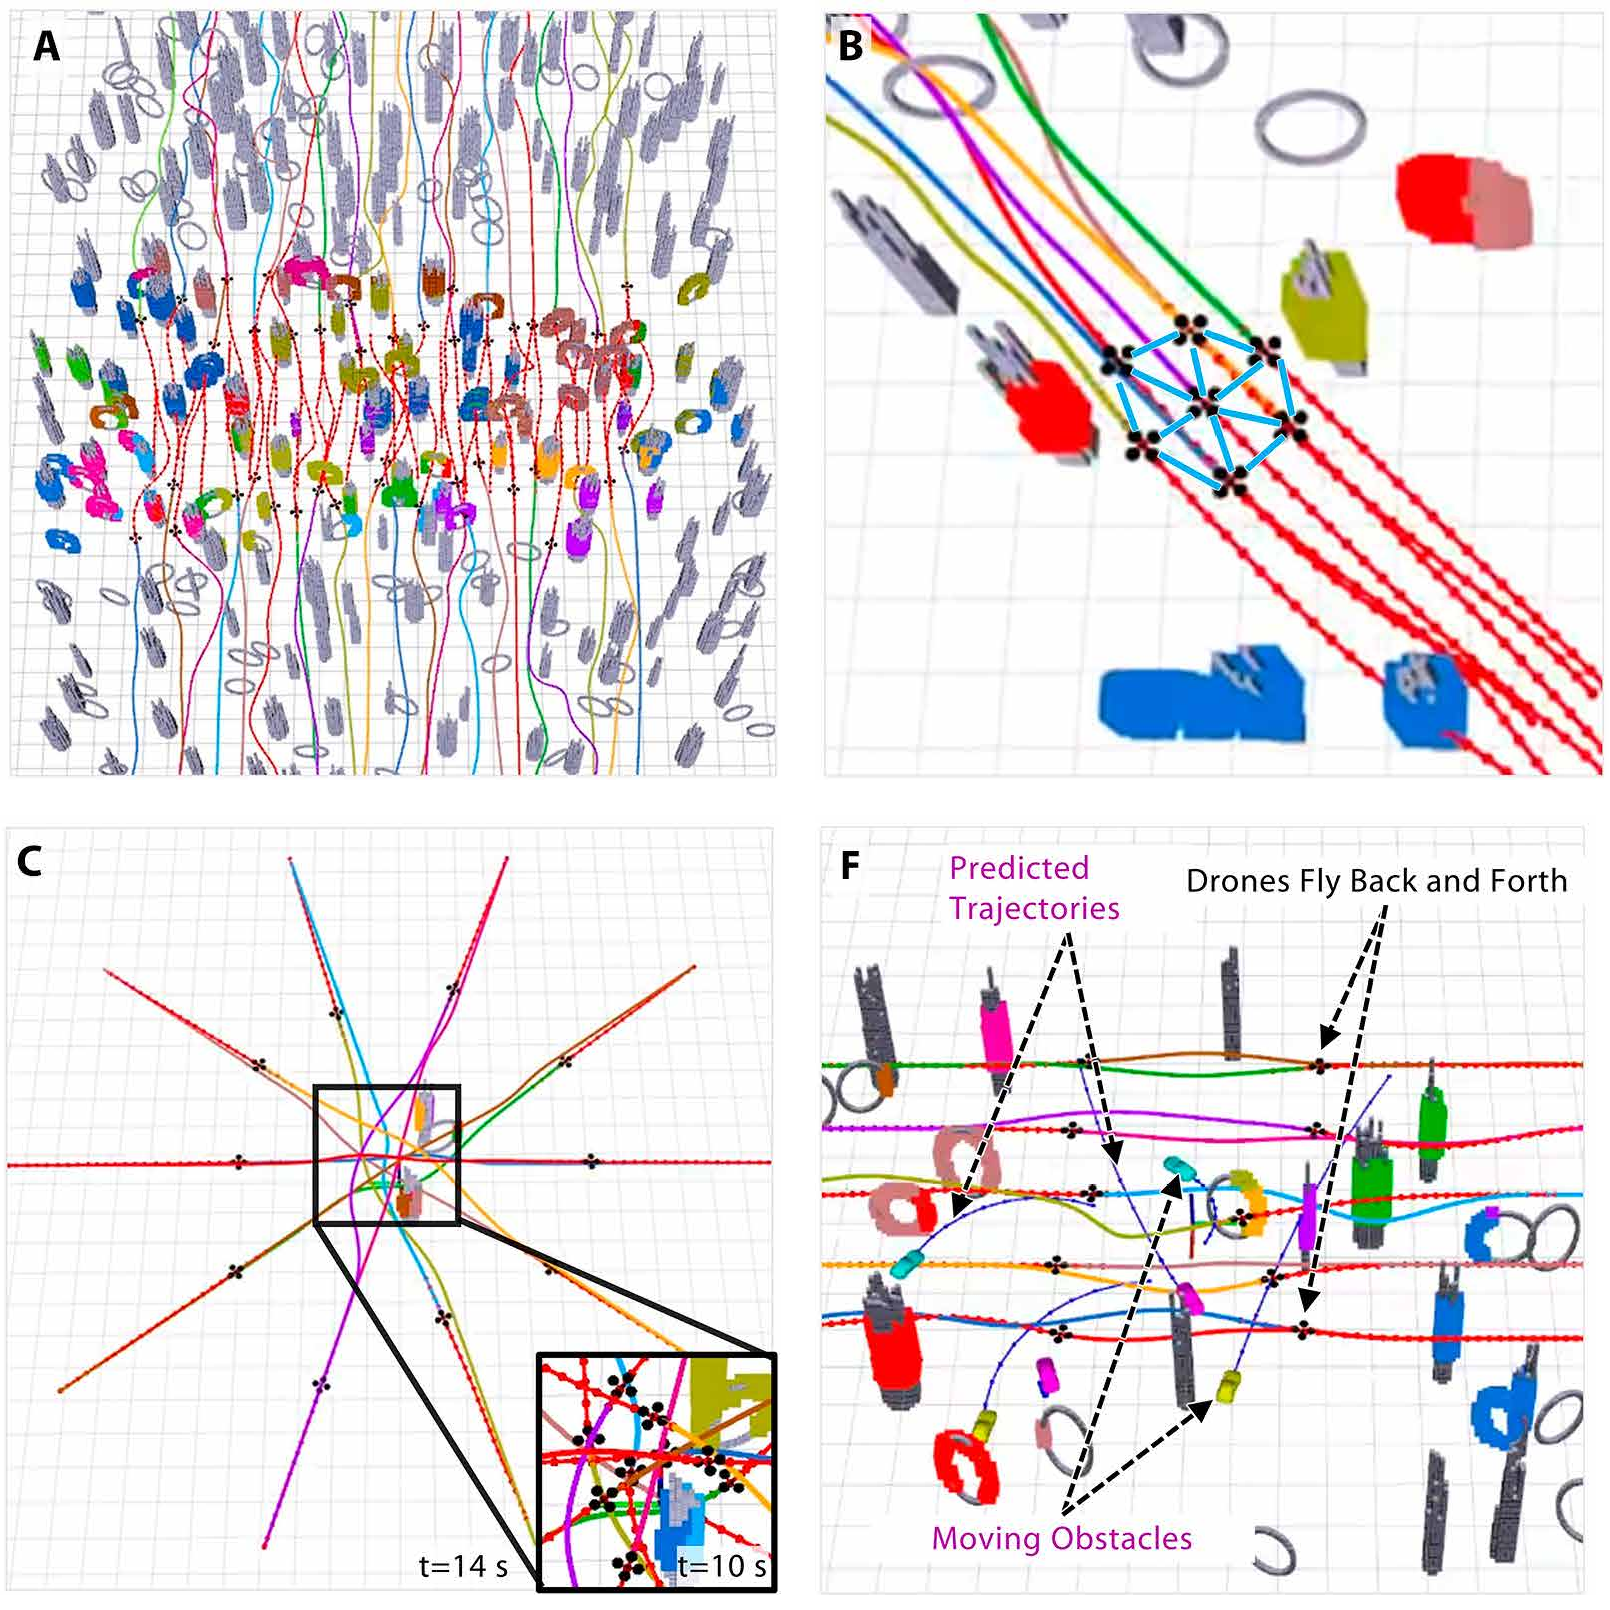
\includegraphics[width=0.91\textwidth]{swarm-playground-comportamentos.png}
\caption[Comportamentos de enxame no swarm playground]{Simulações no \emph{swarm playground}: (A) navegação de 40 drones; (B) formação; (C) troca de posições em um círculo; (F) desvio de obstáculos móveis. As linhas contínuas coloridas representam trajetórias anteriores; as vermelhas com marcadores, trajetórias planejadas; os símbolos pretos, drones; os objetos cinzentos, obstáculos ainda não percebidos; e os coloridos, obstáculos percebidos. Em B, os segmentos cianos indicam a formação. Seleção e reorganização dos painéis A, B, C e F da Figura~8 de Zhou et al.~\cite{wildpaper}, preservando suas letras e separando-os por faixas brancas.}
\label{fig:swarm-playground}
\end{figure}

\subsection{Coordenação em ambientes com passagens}
O projeto \emph{Swarm Simulation}, descrito por Jiahao em 2018, apresenta demonstrações em Gazebo e AirSim~\cite{jiahaoswarm}. A Figura~\ref{fig:jiahao-enxame} mostra robôs terrestres no Gazebo. Embora não represente voo, o exemplo permite discutir um problema comum aos sistemas com vários agentes: coordenar deslocamentos em um espaço compartilhado.

\begin{figure}[htbp]
\centering
\begin{minipage}[c]{0.55\textwidth}
\centering
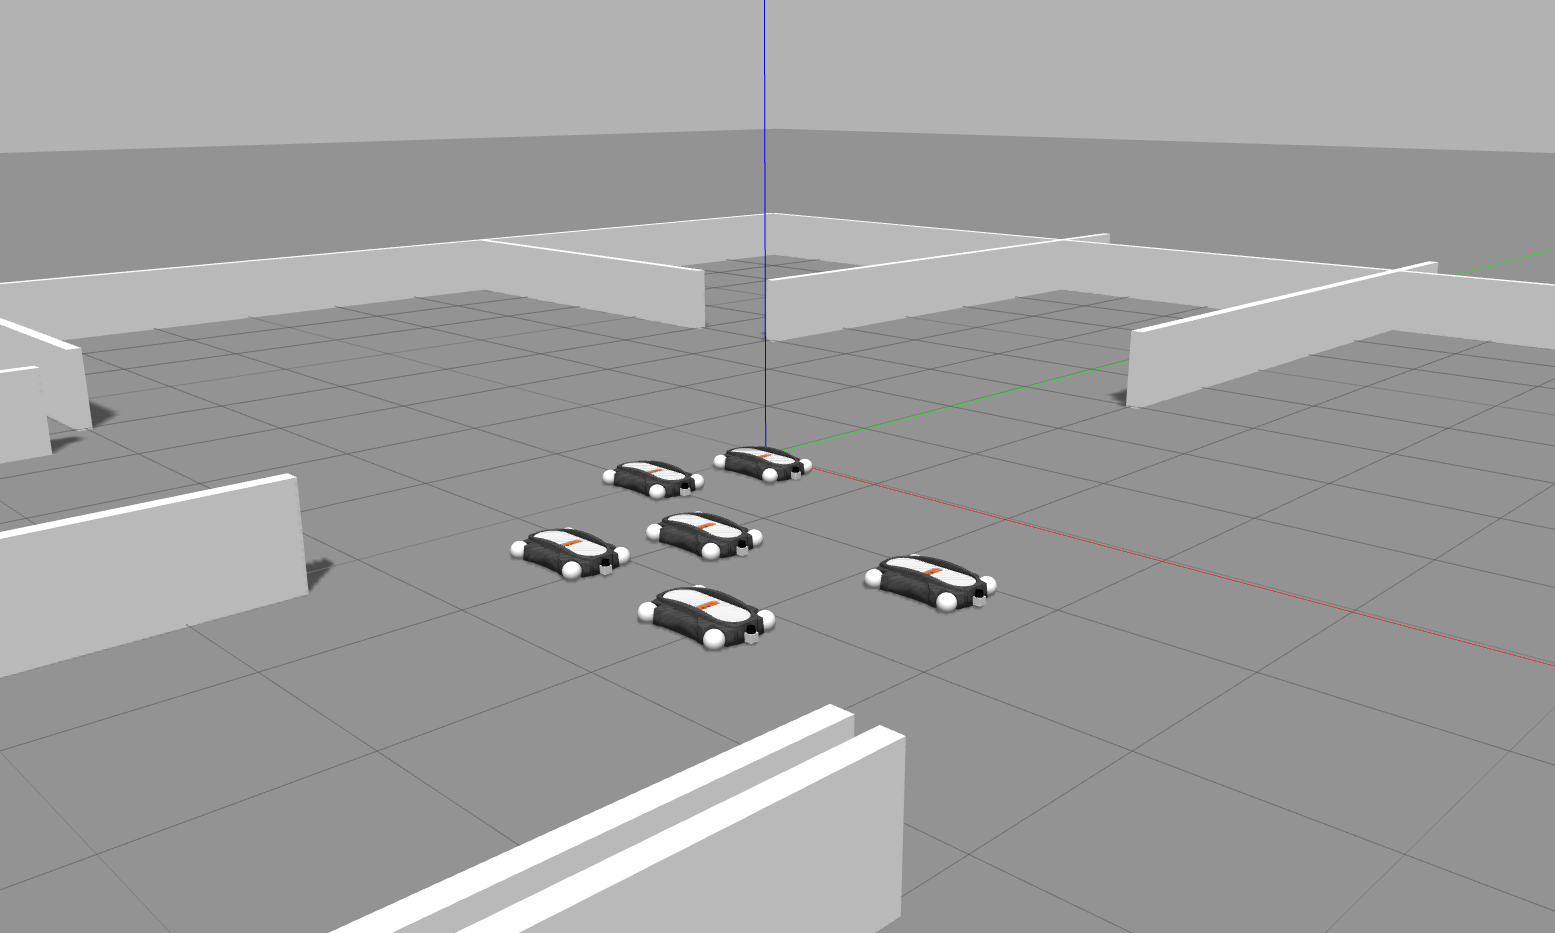
\includegraphics[width=\linewidth]{jiahao-enxame-gazebo.png}
\end{minipage}\hfill
\begin{minipage}[c]{0.42\textwidth}
\centering
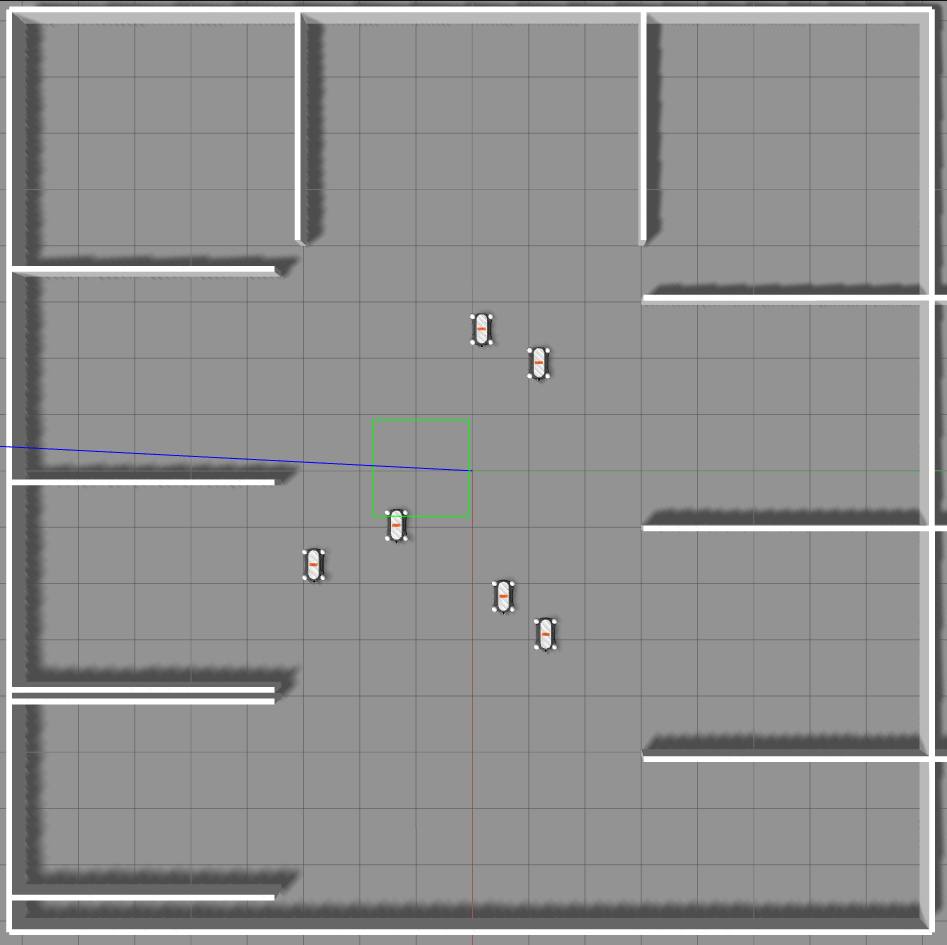
\includegraphics[width=\linewidth]{jiahao-enxame-mapa.png}
\end{minipage}
\caption[Grupo de robôs em ambiente Gazebo com passagens]{Exemplo do projeto \emph{Swarm Simulation}: à esquerda, bases KUKA YouBot em um cenário Gazebo; à direita, vista superior do ambiente com os robôs e uma região delimitada em verde. As paredes definem salas e passagens. As capturas mostram a configuração espacial, sem registrar a evolução temporal do movimento. Reprodução de imagens disponibilizadas por Jiahao~\cite{jiahaoswarm}.}
\label{fig:jiahao-enxame}
\end{figure}

O autor relata bloqueios quando vários robôs recebem o mesmo ponto de destino. A alternativa descrita foi distribuir destinos dentro de uma região, em vez de concentrá-los em uma única posição~\cite{jiahaoswarm}. O caso ilustra como a simulação pode revelar um conflito na definição da tarefa, antes de atribuí-lo ao controle do veículo. As demonstrações em vídeo estão disponíveis na \href{https://www.jiahaoz.com/swarm-simulation}{página do projeto}.

\FloatBarrier
\section{Ferramentas de simulação e integração}
As situações ilustradas exigem representações diferentes conforme o aspecto investigado. Para estudar regras de formação, pode ser suficiente representar posições, velocidades e vizinhanças. Para examinar navegação com câmeras ou respostas do controlador, são necessários modelos de sensores ou da dinâmica da aeronave. A Tabela~\ref{tab:simuladores} relaciona ferramentas a essas funções.

\subsection{Análise da coordenação}
O SwarmLab é um simulador desenvolvido em MATLAB para estudar drones individuais e enxames. Disponibiliza modelos de massa pontual e de quadricóptero, regras de interação e recursos de visualização e análise~\cite{swarmlab,swarmrepo}. Permite examinar a relação entre os parâmetros de coordenação e as trajetórias do grupo. Um modelo de massa pontual, entretanto, não representa diretamente atitude, motores ou dimensões da estrutura. Os exemplos de trajetórias do Capítulo~\ref{cap:casos} complementam essa aplicação.

\subsection{Integração com o software de voo}
Em uma configuração \emph{software-in-the-loop} (SITL), a pilha de voo é executada no computador e conectada a um modelo de veículo. Isso permite examinar comandos, estados e modos de operação antes de conectar uma controladora física. PX4 e ArduPilot documentam esse tipo de execução~\cite{px4sim,ardusitl}.

O Gazebo representa a dinâmica, sensores e objetos do ambiente~\cite{gazebo}. Na integração com PX4, calcula o movimento e fornece informações à pilha de voo, que produz os comandos de controle~\cite{px4gazebo}. Essa organização permite investigar a cadeia entre percepção, planejamento e resposta da aeronave simulada. A presença de um obstáculo na cena só influencia a percepção quando os sensores e o processamento utilizados o representam.

\subsection{Supervisão de missões e integração com a plataforma}
O QGroundControl fornece recursos de configuração, planejamento e acompanhamento de missões~\cite{qgc}. Durante a simulação, pode apresentar estados da pilha de voo e instruções enviadas ao veículo. Sua função é a de estação de solo; o cálculo da dinâmica cabe ao simulador conectado ao sistema.

O Crazyswarm2 documenta recursos de simulação no ecossistema Crazyflie e ROS~2~\cite{crazyswarm2}. Ferramentas vinculadas à plataforma permitem verificar componentes da aplicação e suas interfaces antes da conexão com as aeronaves. É necessário verificar quais interfaces e funções utilizadas na simulação também estão disponíveis nas aeronaves.

\begin{table}[htbp]
\centering\small
\caption{Ferramentas de apoio ao desenvolvimento e atividades descritas em suas documentações.}
\label{tab:simuladores}
\begin{tabularx}{\textwidth}{@{}>{\raggedright\arraybackslash}p{3cm}YY@{}}
\toprule
Ferramenta & Atividade apoiada & Aspecto a verificar \\
\midrule
SwarmLab & Examinar regras de interação e movimento coletivo & Modelo do agente e parâmetros da coordenação \\
Gazebo com PX4 & Examinar voo e navegação em ambiente simulado & Dinâmica, sensores e integração com a pilha de voo \\
ArduPilot SITL & Verificar operação e integração do software de voo & Modelo do veículo e interfaces da aplicação \\
QGroundControl & Configurar, planejar e acompanhar missões & Conexão com a pilha de voo e instruções da missão \\
Crazyswarm2 & Preparar aplicações no ecossistema Crazyflie & Correspondência entre recursos simulados e físicos \\
\bottomrule
\end{tabularx}
\end{table}

\section{Limites dos modelos e transferência para o voo real}\label{sec:limites-sim}
A simulação fornece evidência sobre o comportamento representado pelo modelo. Vibração, ruído dos sensores, interferência de rádio e consumo de energia só participam da avaliação quando são modelados. Mesmo nesses casos, a correspondência com o veículo depende de calibração ou de comparação com medições físicas.

Uma trajetória executada sem colisões no ambiente virtual não estabelece, por si só, a segurança do voo real. A contribuição da simulação está em examinar decisões de coordenação, identificar conflitos e verificar a integração de software. Os aspectos físicos que ela não representa precisam ser avaliados na plataforma escolhida.


%######################################################################
\chapter{Estudos de caso}\label{cap:casos}
Os quatro exemplos a seguir investigam condições diferentes e não podem ser comparados apenas pela quantidade de drones (ver Tabela~\ref{tab:eixos}). A seleção ilustra como os conceitos das seções anteriores se combinam em sistemas reais.

\section{Crazyswarm: laboratório com localização externa}\label{sec:crazy}
Preiss et al. construíram uma plataforma para coordenar até 49 Crazyflies em ambiente interno. Uma estação recebeu medições de captura de movimento e transmitiu informações de posição por três rádios. Cada aeronave executou estimação, avaliação de trajetória e controle a bordo, com ciclo embarcado a 500~Hz nas condições descritas no artigo~\cite{crazyswarm}. As Figuras~\ref{fig:plataforma-crazy} e~\ref{fig:estudo-crazy} mostram o veículo e o ambiente experimental.

\begin{figure}[htbp]
\centering
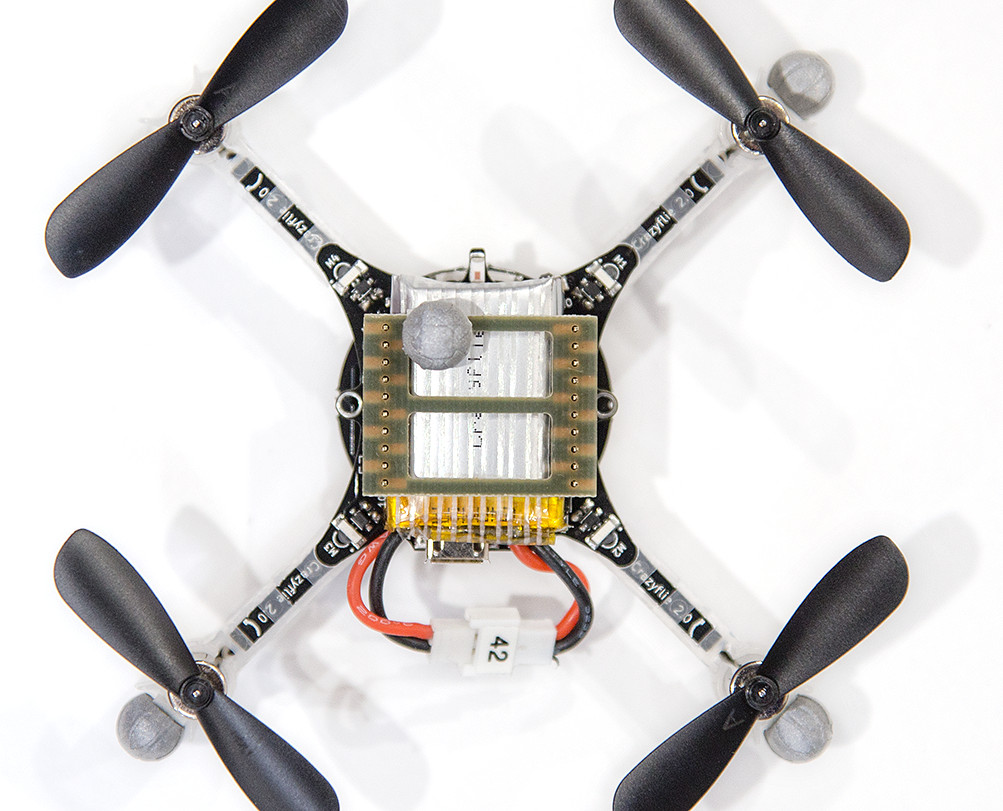
\includegraphics[width=0.35\textwidth]{crazyswarm-plataforma.jpg}
\caption[Crazyflie utilizado no estudo Crazyswarm]{Crazyflie~2.0 com bateria e marcadores de captura de movimento. Reprodução da Fig.~1 de Preiss et al.~\cite{crazyswarm}.}
\label{fig:plataforma-crazy}
\end{figure}

\begin{figure}[htbp]
\centering
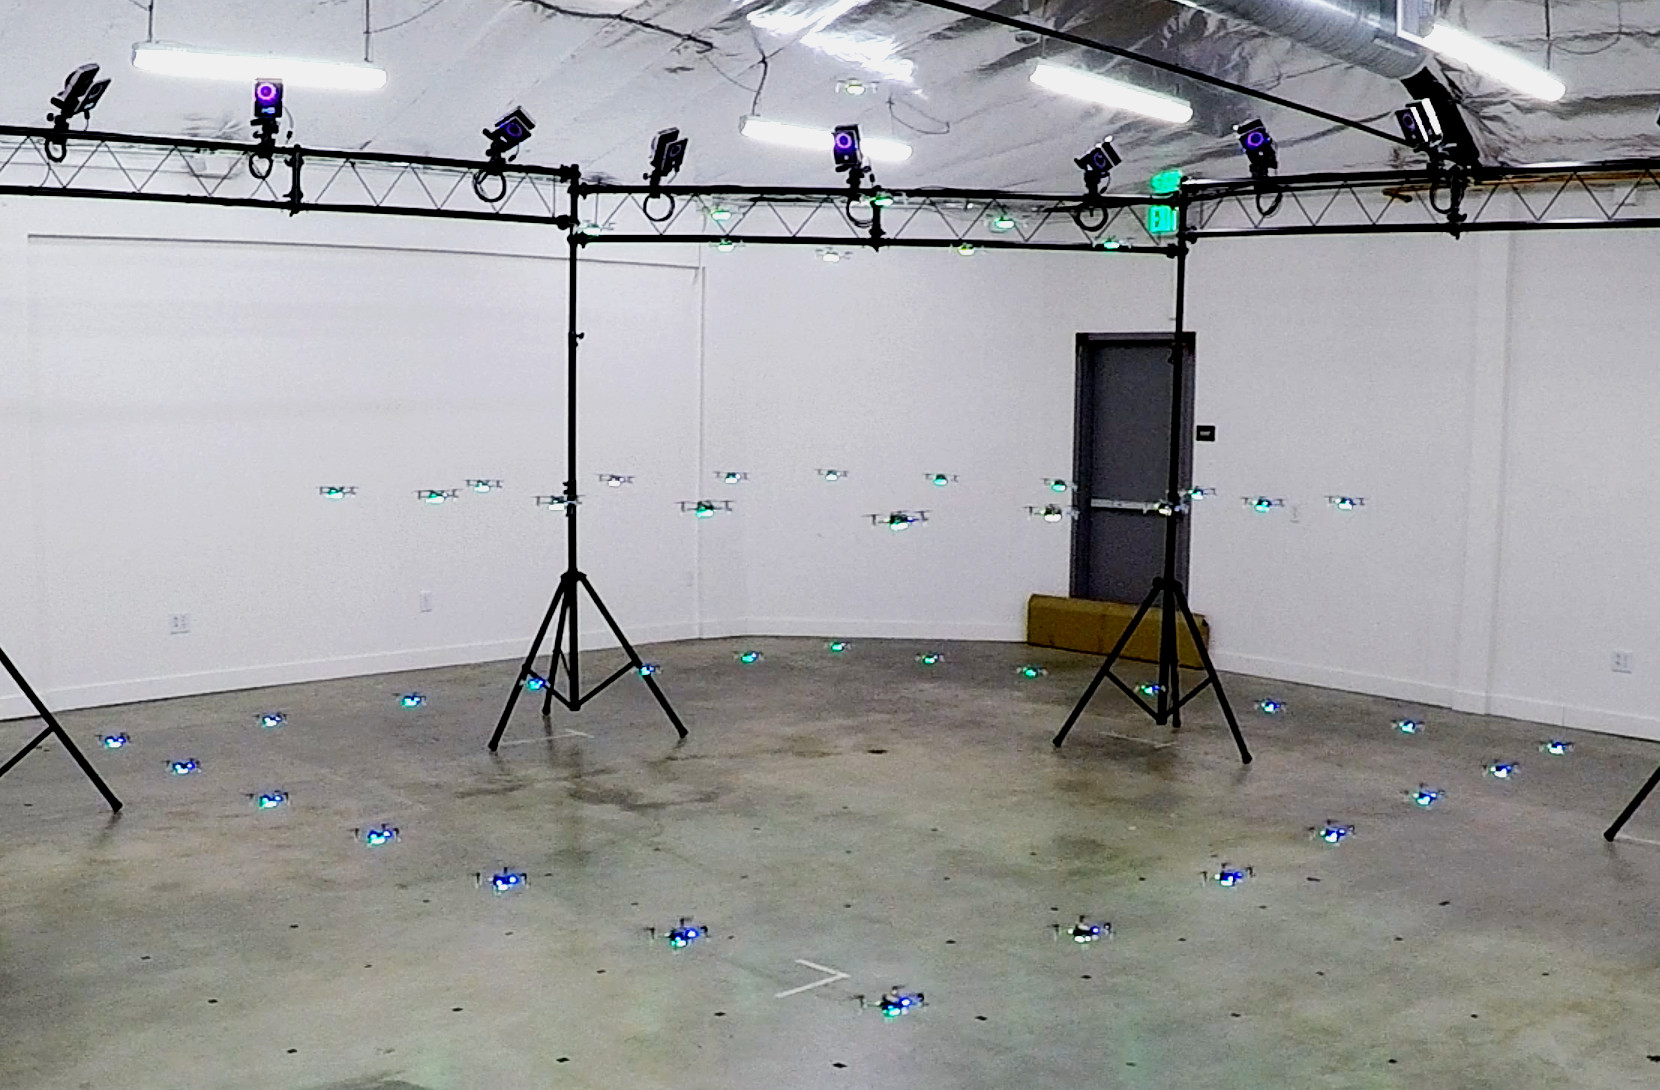
\includegraphics[width=0.73\textwidth]{crazyswarm-experimento.jpg}
\caption[Experimento interno com a plataforma Crazyswarm]{Ambiente experimental do Crazyswarm, com nanoquadricópteros e câmeras de captura de movimento. Fotografia extraída de Preiss et al.~\cite{crazyswarm}, p.~6.}
\label{fig:estudo-crazy}
\end{figure}

O exemplo permite distinguir controle embarcado de localização embarcada: os cálculos de controle foram executados nas aeronaves, mas a localização utilizou câmeras externas. A fotografia da Figura~\ref{fig:plataforma-crazy} corresponde à configuração do estudo de 2017, e não à Crazyflie Brushless citada no Capítulo~\ref{cap:eletr}. Transferir essa arquitetura para um local sem captura de movimento exige substituir a fonte de localização e avaliar novamente o sistema.

\section{Navegação de dez drones em uma floresta de bambu}
Zhou et al. avaliaram dez drones em uma floresta de bambu, com um destino situado 65~m à frente, fora da floresta. O planejador ajustou o movimento no espaço e no tempo para contornar obstáculos e compatibilizar a passagem dos agentes por regiões estreitas~\cite{wildpaper}. O código do planejador (EGO-Planner-v2) foi disponibilizado pelos autores~\cite{wildcode}. A Figura~\ref{fig:estudo-floresta} reúne registros do voo e o mapa associado às trajetórias.

\begin{figure}[htbp]
\centering
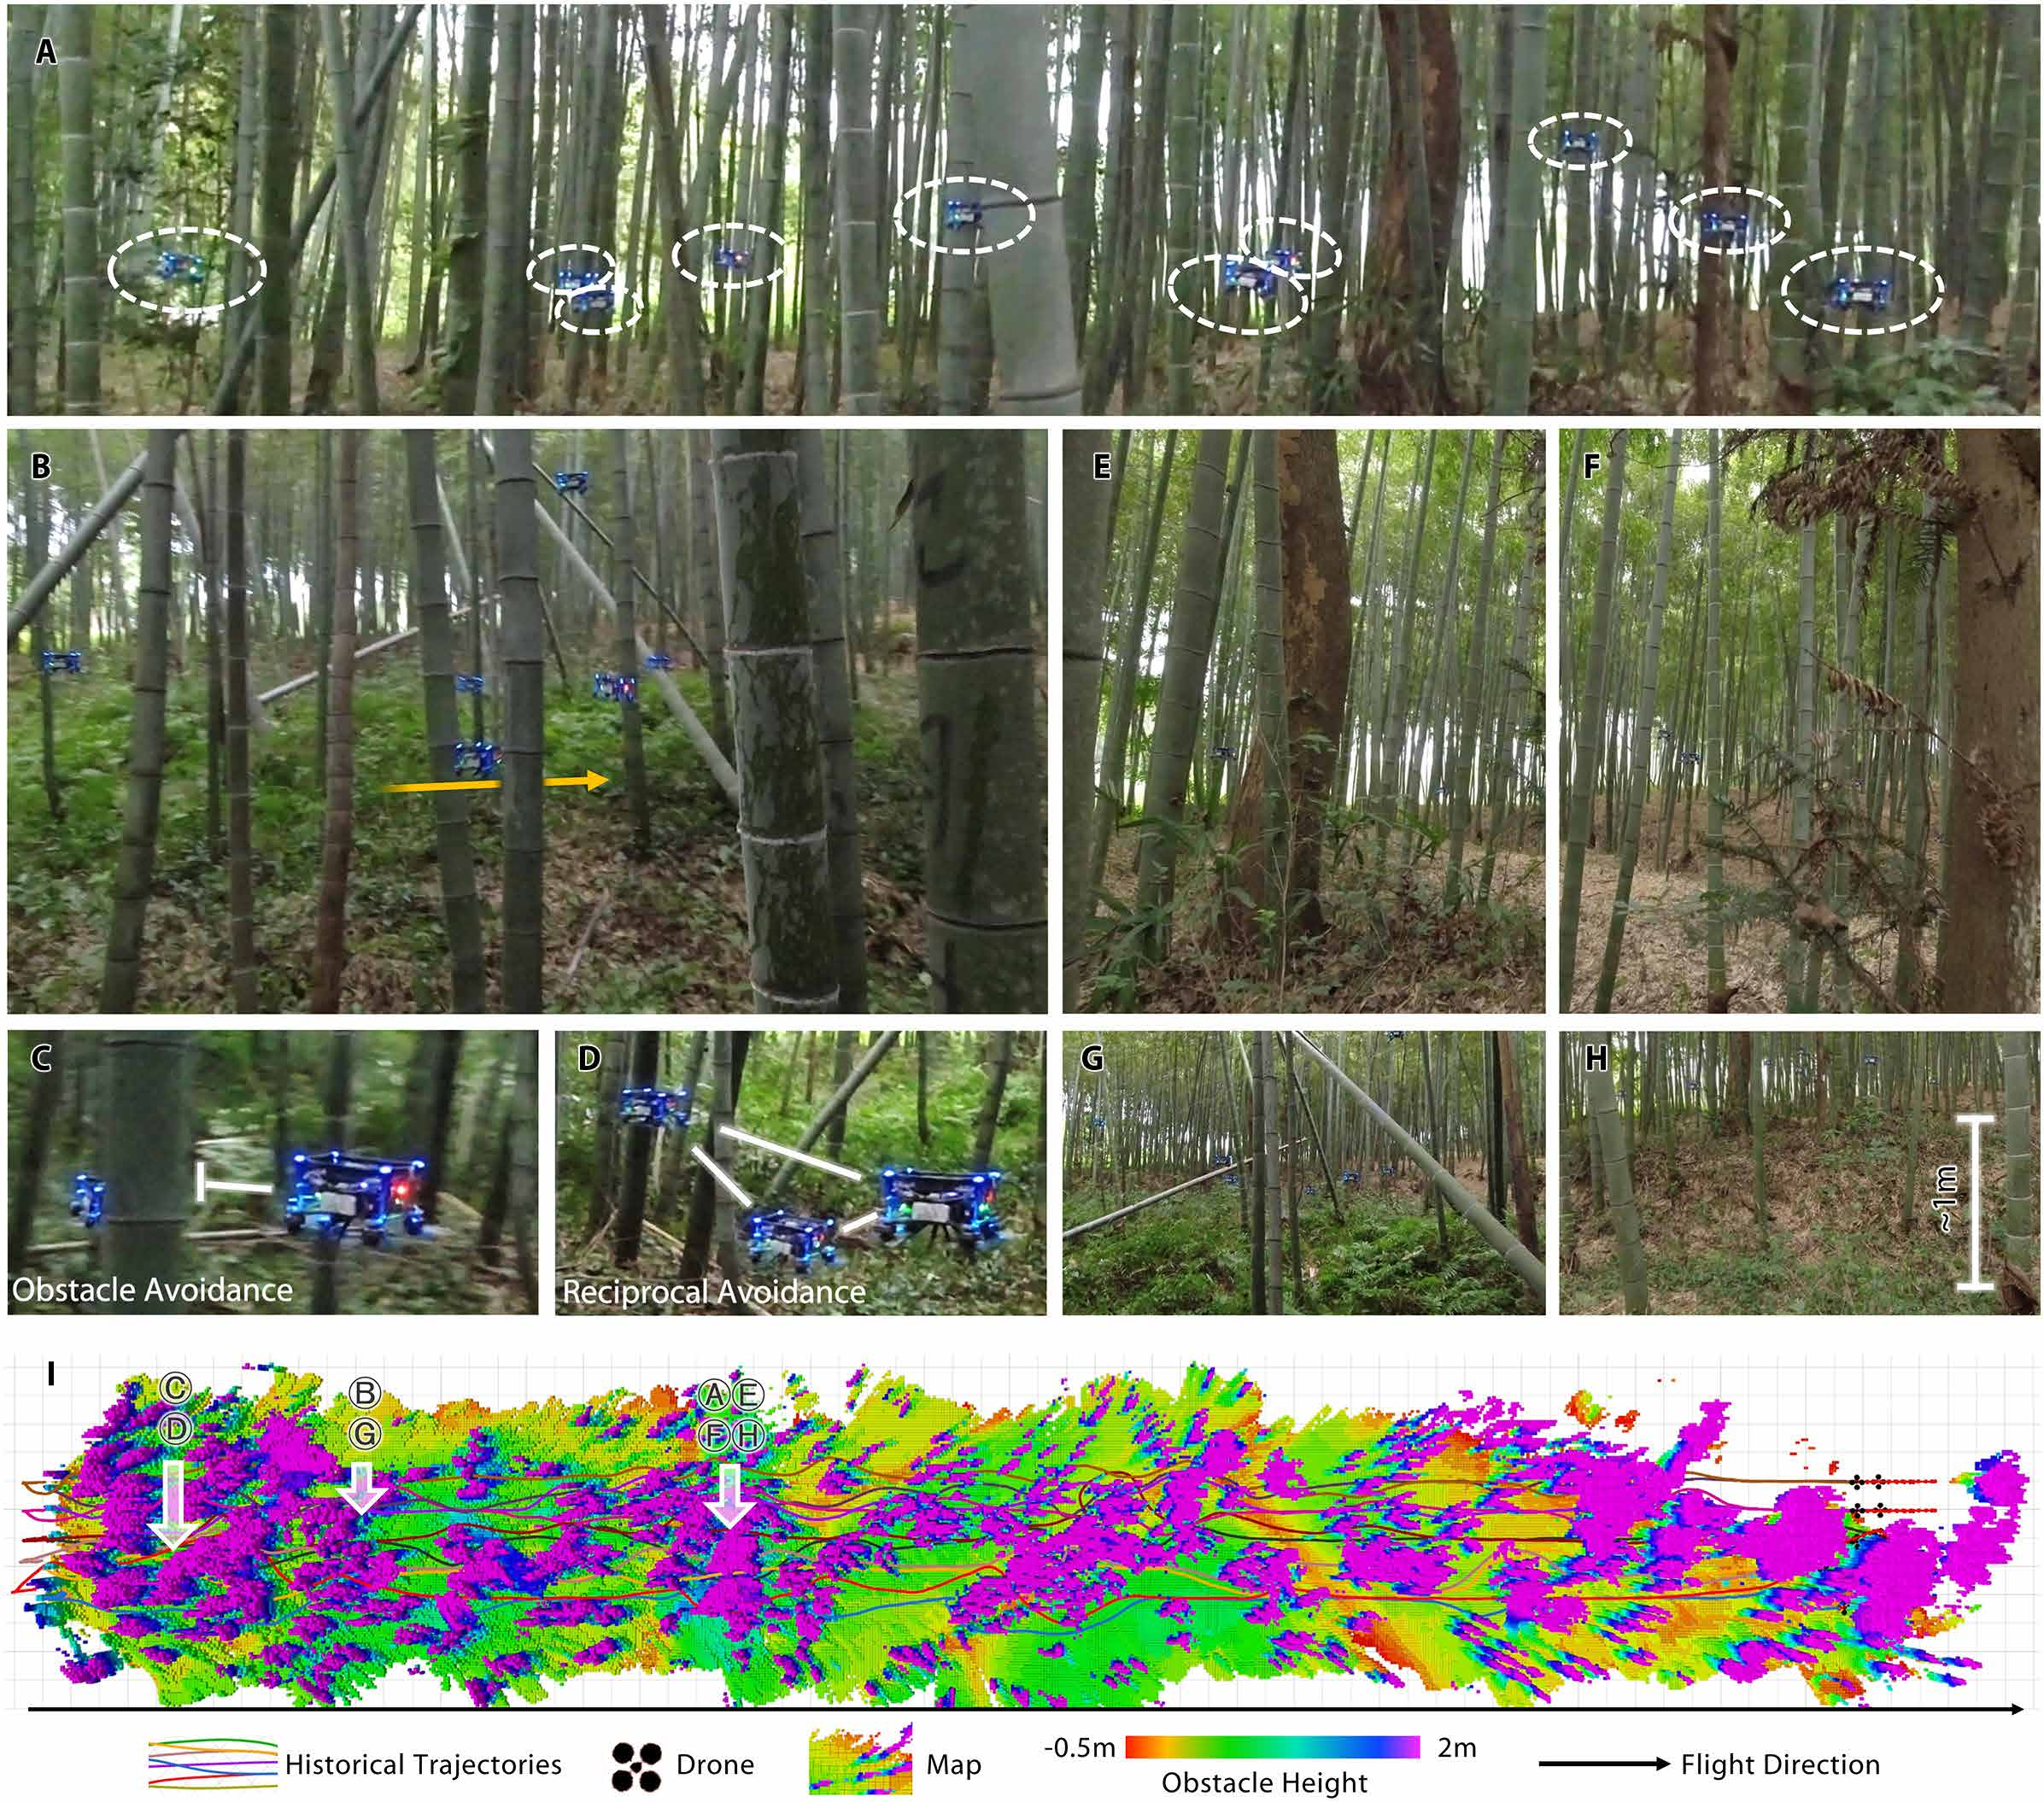
\includegraphics[width=0.88\textwidth,height=0.48\textheight,keepaspectratio]{enxame-floresta-experimento.jpg}
\caption[Navegação de dez drones em floresta de bambu]{Experimento de navegação na floresta. Os painéis mostram o enxame, passagens estreitas, desvio de obstáculos, interação entre drones e condições do terreno; o painel inferior apresenta o mapa e as trajetórias registradas. Reprodução da Fig.~3 de Zhou et al.~\cite{wildpaper}, sem alteração.}
\label{fig:estudo-floresta}
\end{figure}

O exemplo conecta percepção e planejamento: a câmera fornece informações sobre o ambiente, a estimação fornece o estado do veículo e o planejador atualiza a trajetória. A observação de voo entre bambus sustenta a operação nas condições do experimento; não estabelece desempenho equivalente sob outras condições de iluminação, vegetação ou comunicação. Reproduzir o experimento exige integrar os subsistemas descritos pelos autores; os critérios para planejar esse esforço são discutidos no Capítulo~\ref{cap:plat}.

\section{SwarmLab: trajetórias e métricas em simulação}
Soria et al. desenvolveram o SwarmLab para simular e comparar comportamentos coletivos. O artigo avaliou algoritmos de Olfati-Saber e Vásárhelyi por métricas de movimento e organização do grupo~\cite{swarmlab}. A documentação fornece os exemplos das Figuras~\ref{fig:estudo-swarm-traj} e~\ref{fig:estudo-swarm-dist}~\cite{swarmrepo}.

\begin{figure}[htbp]
\centering
\begin{minipage}[t]{0.48\textwidth}
\centering
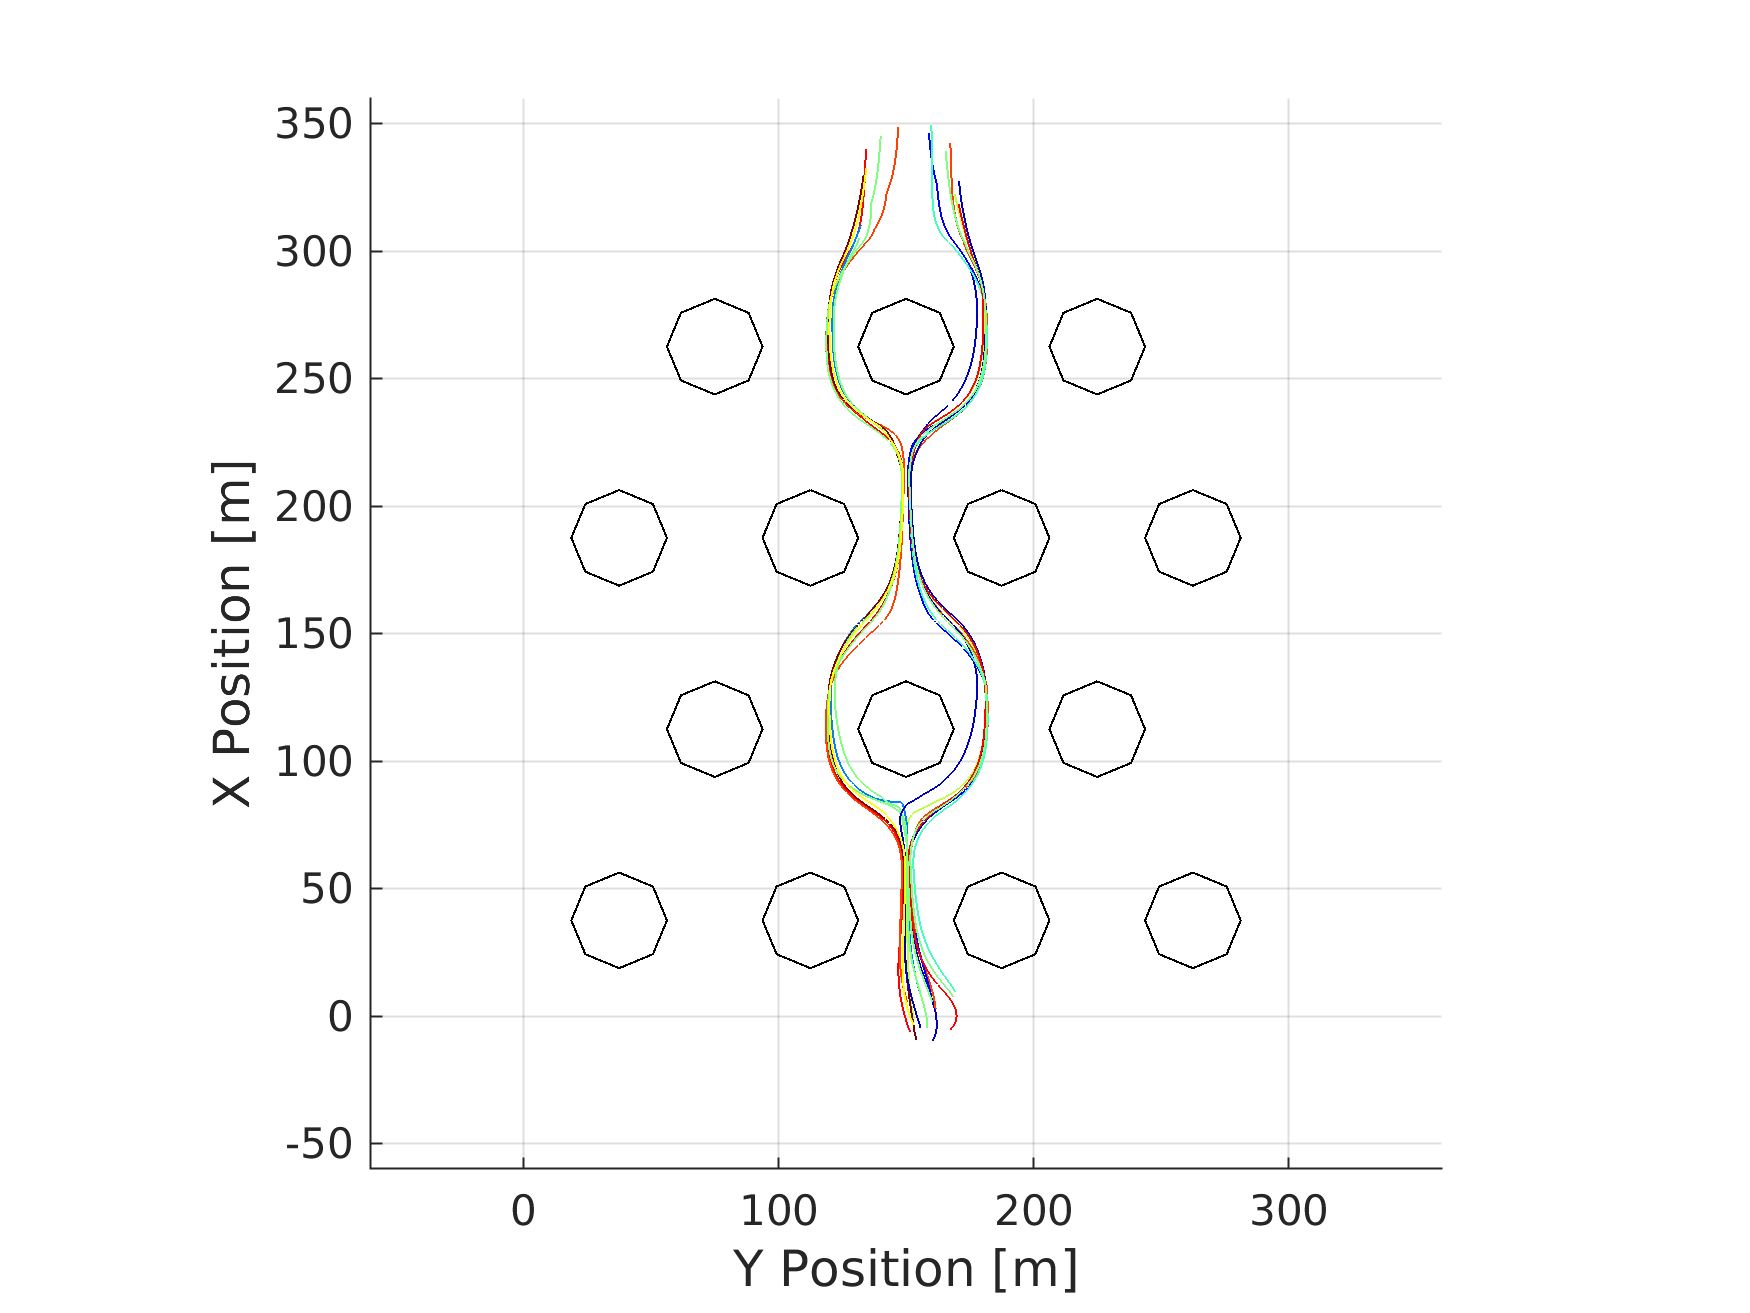
\includegraphics[width=\linewidth]{swarmlab-trajetorias.png}
\caption[Trajetórias simuladas no SwarmLab]{Trajetórias simuladas na documentação do SwarmLab~\cite{swarmrepo}. As curvas coloridas representam trajetórias; os contornos pretos, obstáculos. Posições em metros.}
\label{fig:estudo-swarm-traj}
\end{minipage}\hfill
\begin{minipage}[t]{0.48\textwidth}
\centering
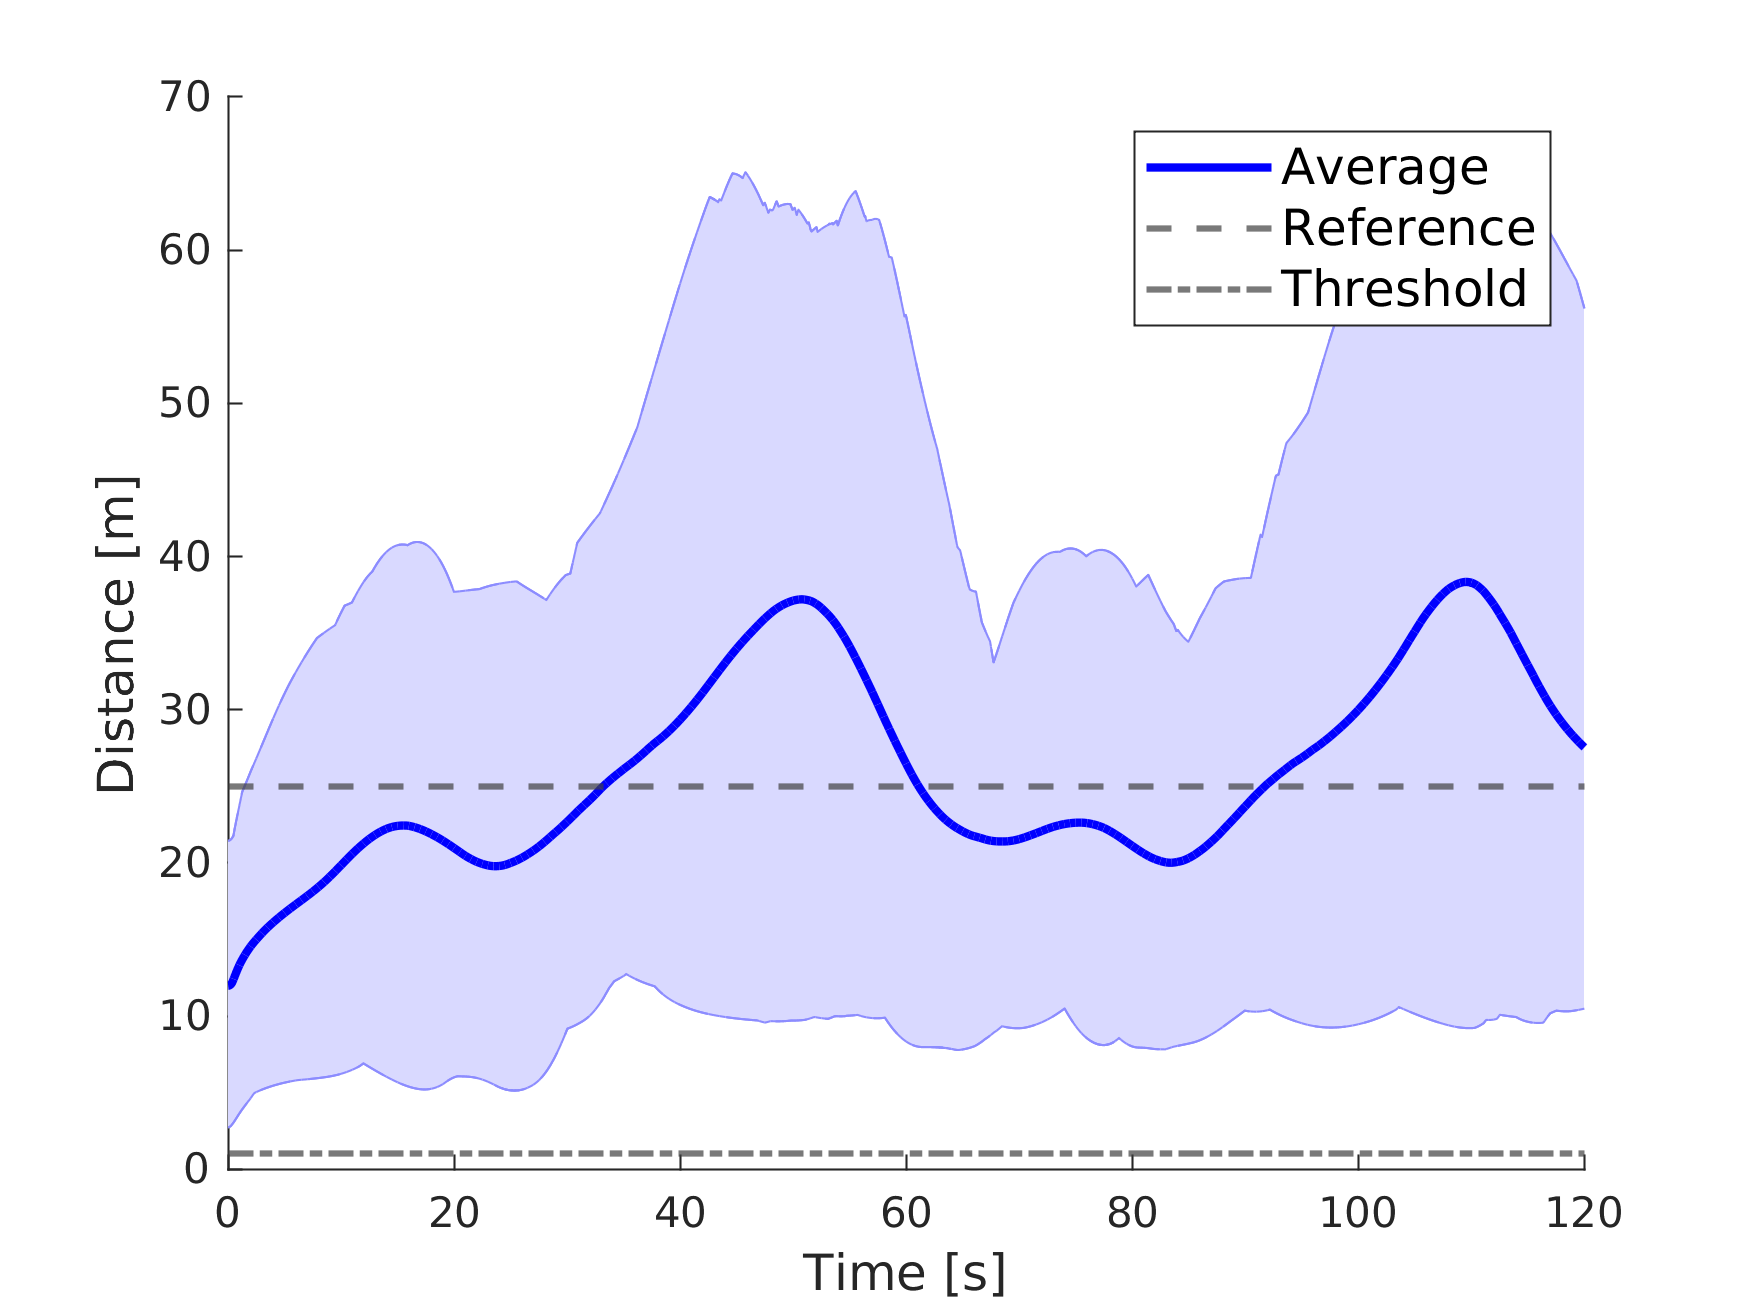
\includegraphics[width=\linewidth]{swarmlab-distancias.png}
\caption[Distâncias entre agentes na documentação do SwarmLab]{Distâncias entre agentes na documentação do SwarmLab~\cite{swarmrepo}, com rótulos e escalas originais.}
\label{fig:estudo-swarm-dist}
\end{minipage}
\end{figure}

O contorno dos obstáculos mostra onde o grupo muda de direção, mas a imagem de trajetórias não quantifica, isoladamente, a separação entre agentes. Para avaliar essa separação, o pesquisador precisa registrar distâncias ao longo do tempo e compará-las com o tamanho dos veículos e a margem adotada. Os gráficos reproduzem exemplos dos autores e não foram gerados por simulações executadas para este livro; como a documentação não identifica todos os parâmetros do exemplo, sua reprodução é limitada.

\section{SGBA: exploração com recursos limitados}
O Swarm Gradient Bug Algorithm (SGBA), descrito por McGuire, combina avanço em uma direção, acompanhamento de contornos de obstáculos e retorno ao ponto de partida. A plataforma utiliza sensores de distância, fluxo óptico e rádio, com processamento no microcontrolador do veículo~\cite{mcguire}. A descrição consultada é o capítulo da tese da autora; os dados do artigo associado são disponibilizados pelo laboratório~\cite{dados}, cujo texto integral não foi consultado.

O exemplo ilustra uma escolha diferente da navegação com mapa: a tarefa é explorar e retornar, e o sistema combina comportamentos sem construir um mapa convencional. A avaliação precisa, portanto, considerar cobertura e retorno, além da forma da trajetória. Pela descrição consultada, o método não oferece deslocamento preciso a qualquer posição do ambiente.

\section{Síntese das arquiteturas e condições de avaliação}
O Crazyswarm combina controle embarcado e localização externa. O trabalho na floresta integra percepção e planejamento a bordo. O SwarmLab permite variar modelos e regras de interação em simulação. O SGBA explora a navegação com sensores e computação limitados. A revisão sobre microveículos aéreos organiza as restrições que atravessam essas escolhas~\cite{survey}; ela é uma fonte de classificação conceitual, e não um experimento adicional.

%######################################################################
\chapter[Escolha de plataformas]{Escolha de plataformas conforme o objetivo de pesquisa}\label{cap:plat}
A escolha da plataforma depende da variável investigada e do esforço de engenharia que a equipe pode assumir. A miniaturização restringe massa, energia e espaço e pode aumentar o trabalho de integração. O custo e o risco físico precisam ser avaliados para a configuração e as condições de operação previstas.

\section{Critérios de seleção da plataforma}
Os critérios principais são: (i) o objetivo de pesquisa (algoritmo de coordenação, estimação, controle ou percepção); (ii) o número de agentes; (iii) o ambiente (interno ou externo, confinado ou aberto); (iv) onde ficam a percepção e a computação (a bordo ou externas); (v) os requisitos de segurança; e (vi) o orçamento e o tempo de engenharia disponíveis.

\section{Configurações experimentais e fontes de complexidade}
A Tabela~\ref{tab:niveis} organiza quatro configurações experimentais. As configurações distinguem fontes de dificuldade, mas não constituem uma sequência obrigatória. O esforço depende da experiência da equipe, dos componentes utilizados e do grau de intervenção no sistema. A Seção~\ref{sec:competencias} relaciona essas escolhas aos conhecimentos necessários.

\begin{table}[htbp]
\centering\small
\caption{Configurações experimentais para pesquisa com drones. A numeração organiza a exposição e não indica uma ordem obrigatória de dificuldade.}
\label{tab:niveis}
\begin{tabularx}{\textwidth}{@{}>{\raggedright\arraybackslash}p{3cm}YY@{}}
\toprule
Configuração & O que se investiga & Plataforma típica \\
\midrule
0. Simulação & Modelagem, controle, navegação e sensibilidade a parâmetros & SwarmLab; SITL do PX4 ou ArduPilot \\
1. Laboratório com localização externa & Controle e trajetórias com referência externa de posição & Nanoquadricópteros (Crazyflie) com captura de movimento \\
2. Plataforma média e aberta & Sensores, cargas úteis, controle próprio e processamento embarcado & Estruturas de classe F450 ou X500 com controladora compatível com PX4 ou ArduPilot \\
3. Micro com percepção embarcada & Navegação sem infraestrutura externa, com computação a bordo & Montagem própria otimizada em massa e consumo \\
\bottomrule
\end{tabularx}
\end{table}

\section{Porte da aeronave e restrições de integração}
Uma estrutura de classe F450, com distância entre eixos de cerca de 450~mm, pode facilitar a instalação de controladora, computador complementar, câmera, receptor de navegação por satélite, rádio e fiação. O espaço disponível favorece o acesso a conectores e portas durante o diagnóstico. A carga admissível depende do dimensionamento da propulsão e da alimentação. O porte das hélices e a energia envolvida no voo também precisam orientar as condições de teste. Neste capítulo, esse porte é considerado para integrar sensores, cargas úteis, algoritmos de controle e computadores embarcados em uma aeronave. A operação em grupo acrescenta requisitos de espaço, baterias, manutenção e pessoal. O Holybro X500~V2, usado como exemplo na Seção~\ref{sec:dji-diy}, pertence a uma classe semelhante.

Drones de menor porte, como os usados na floresta de bambu~\cite{wildpaper}, permitem estudar a navegação por passagens estreitas. Sua integração exige conciliar sensores, processamento e bateria com limites de massa, consumo e espaço. A fiação e a disposição dos componentes também precisam ser avaliadas quanto à vibração, à distribuição de massa e à dissipação térmica. O tempo de voo e os efeitos de uma colisão dependem da configuração e das condições de operação; o porte, isoladamente, não permite quantificá-los. O artigo e seu material suplementar descrevem a plataforma utilizada no experimento~\cite{wildpaper}.

\begin{table}[htbp]
\centering\small
\caption{Restrições de integração em plataformas de porte médio e micro com percepção embarcada. Os itens indicam aspectos a verificar em cada configuração.}
\label{tab:f450-micro}
\begin{tabularx}{\textwidth}{@{}>{\raggedright\arraybackslash}p{3cm}YY@{}}
\toprule
Critério & Classe F450 & Micro com percepção embarcada \\
\midrule
Espaço e carga útil & Verificar espaço e carga admissível & Conciliar componentes com limites de massa e espaço \\
Esforço de integração & Espaço pode facilitar o uso de módulos comerciais & Miniaturização pode exigir peças e arranjo próprios \\
Segurança em teste & Considerar massa, velocidade e porte das hélices & Avaliar os mesmos fatores e a proteção necessária \\
Custo por unidade & Orçar componentes e integração & Incluir o esforço de miniaturização \\
Operação em grupo & Planejar espaço, baterias e pessoal & Avaliar repetibilidade da montagem e suporte ao grupo \\
Ambientes confinados & Verificar dimensões e margens de passagem & Menor porte pode permitir passagens mais estreitas \\
Diagnóstico & Espaço pode facilitar acesso aos componentes & Acesso aos componentes pode ser limitado \\
\bottomrule
\end{tabularx}
\end{table}

\section{Componentes de uma plataforma experimental}
A escolha dos materiais parte da variável que a pesquisa pretende modificar. Experimentos sobre coordenação com localização externa podem utilizar plataformas menores; experimentos sobre percepção embarcada exigem capacidade de processamento, sensores e alimentação compatíveis. A Tabela~\ref{tab:materiais} organiza opções por função, sem constituir uma lista de compra validada.

\begin{table}[htbp]
\centering\small
\caption{Materiais e recursos para especificar uma plataforma experimental. As escolhas dependem da tarefa, da massa e das interfaces do veículo.}
\label{tab:materiais}
\begin{tabularx}{\textwidth}{@{}>{\raggedright\arraybackslash}p{3cm}YY@{}}
\toprule
Função & Opções de estudo & Critério de seleção \\
\midrule
Plataforma aérea & Nanoquadricóptero aberto ou montagem própria & Acesso ao software e capacidade de transportar a carga experimental \\
Controle de voo & Controladora compatível com PX4 ou placa aberta da plataforma & Interfaces, registro de dados e possibilidade de modificar o controle \\
Percepção & Câmera, sensor de distância ou localização externa & Campo de visão, taxa de medição, calibração e ambiente \\
Processamento & Microcontrolador ou computador complementar & Tempo de cálculo, consumo, massa e dissipação térmica \\
Comunicação & Rádio da plataforma ou rede entre computadores & Atraso, perdas, número de agentes e volume de mensagens \\
Estrutura & Estrutura original ou peças fabricadas para o protótipo & Massa, rigidez, vibração, reparabilidade e proteção dos componentes \\
Validação & Simulador e registro de estados e comandos & Modelo do veículo, parâmetros e condições reproduzíveis \\
\bottomrule
\end{tabularx}
\end{table}

A Crazyflie é uma opção comercial de desenvolvimento com software aberto e interfaces de expansão documentadas~\cite{bitcraze}, o que mostra que ``comercial'' e ``fechado'' não são sinônimos. Uma montagem \emph{do it yourself} (DIY), por sua vez, reúne componentes selecionados e integrados pelo pesquisador, e o grau de acesso depende de cada componente e de seu software. Para a estrutura mecânica, a escolha entre peças de catálogo, compósitos e polímeros fabricados para o projeto exige ensaios de massa, rigidez e vibração; este levantamento não comparou propriedades de materiais estruturais e não estabelece um material preferencial.

\section{Integração e acesso ao software: exemplos DJI e DIY}\label{sec:dji-diy}
A comparação precisa considerar o nível de intervenção exigido pelo experimento. Um kit de desenvolvimento de software (SDK, do inglês \emph{Software Development Kit}) reúne ferramentas e bibliotecas para desenvolver aplicações. Uma interface de programação de aplicações (API, do inglês \emph{Application Programming Interface}) define como um programa acessa funções de outro sistema.

O Onboard SDK da DJI disponibiliza telemetria e funções de controle em aeronaves compatíveis, com suporte específico por produto~\cite{dji}. A disponibilidade de comandos de posição ou atitude não equivale ao acesso para substituir os controladores internos. Esses controladores fazem parte do firmware, o software embarcado que executa as funções do dispositivo.

A Figura~\ref{fig:plataformas-comparadas} apresenta o DJI Matrice~300~RTK como plataforma integrada e o Holybro X500~V2 com Pixhawk~6C como exemplo de montagem modular com pilha aberta; o X500 é um kit comercial para montagem pelo usuário~\cite{m300imagem,x500imagem}.

\begin{figure}[htbp]
\centering
\begin{minipage}[b]{0.48\textwidth}
\centering
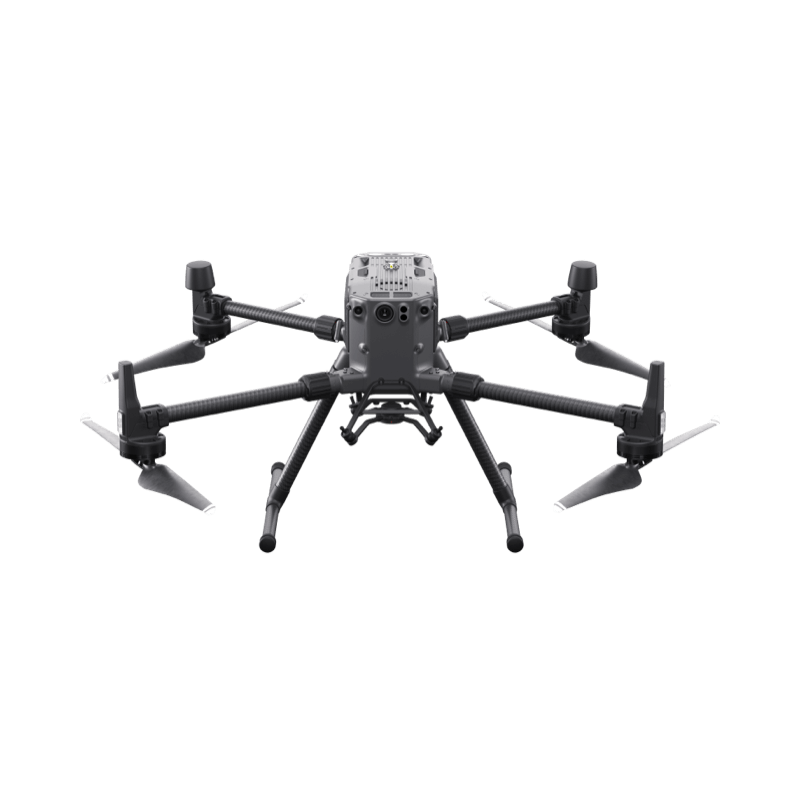
\includegraphics[width=\linewidth,height=3.3cm,keepaspectratio,trim=35 180 35 215,clip]{dji-matrice-300-rtk.png}
\par\smallskip
{\small (a) DJI Matrice~300~RTK}
\end{minipage}\hfill
\begin{minipage}[b]{0.48\textwidth}
\centering
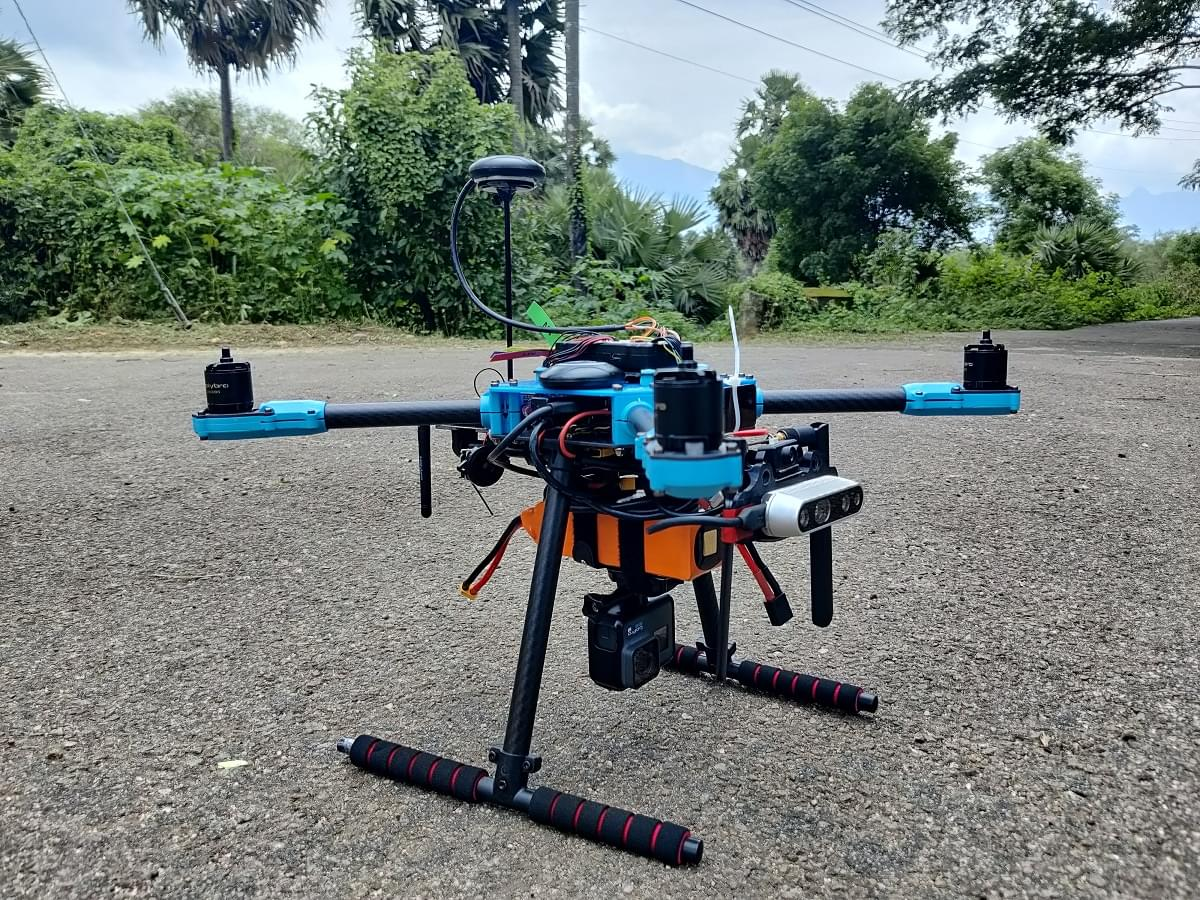
\includegraphics[width=\linewidth,height=3.3cm,keepaspectratio]{holybro-x500-v2.jpg}
\par\smallskip
{\small (b) Holybro X500~V2 com Pixhawk~6C}
\end{minipage}
\caption[Plataformas DJI e modular para comparação]{(a) Matrice~300~RTK, imagem oficial da DJI~\cite{m300imagem}; (b) X500~V2 montado, sem hélices, em fotografia da documentação PX4~\cite{x500imagem}. Imagens em escalas distintas; as margens vazias do painel (a) foram omitidas.}
\label{fig:plataformas-comparadas}
\end{figure}

\begin{table}[htbp]
\centering\small
\caption{Critérios de integração para pesquisa, organizados a partir das interfaces documentadas de cada plataforma.}
\label{tab:comparacao}
\begin{tabularx}{\textwidth}{@{}>{\raggedright\arraybackslash}p{2.8cm}YY@{}}
\toprule
Critério & DJI com interface compatível & DIY com pilha aberta \\
\midrule
Integração inicial & Subsistemas fornecidos como plataforma integrada; a extensão depende do SDK & Permite escolher componentes; exige montagem, calibração e integração \\
Acesso ao controle & Restrito às funções expostas para o produto & Permite alterar o código disponível da pilha e compilar versões experimentais \\
Sensores & Integração condicionada às portas, cargas e APIs suportadas & Seleção de sensores e conexões condicionada ao hardware e aos drivers \\
Reprodução & Depende da combinação de aeronave, firmware e SDK & Pode fixar código e componentes; exige documentar a montagem e as calibrações \\
Manutenção & Depende das peças e do suporte da plataforma & Permite substituições modulares; cada alteração pode exigir nova avaliação \\
Custo & Incluir aeronave, acessórios e interfaces necessárias & Incluir peças, reposições, instrumentação e trabalho de integração \\
\bottomrule
\end{tabularx}
\end{table}

Como recomendação de projeto, uma plataforma integrada pode atender a pesquisas de missão ou de aquisição de dados quando as interfaces expõem os comandos necessários. Para investigar controladores internos, alocação de motores ou modificações na estimação, o acesso ao código torna uma plataforma aberta mais adequada. O PX4 documenta sua arquitetura de controle~\cite{controle}.

\FloatBarrier
\subsection{Massa e miniaturização: DJI Mini 3 e montagem DIY}\label{sec:sub250}
A comparação de plataformas leves é relevante para enxames que precisam atravessar espaços estreitos ou operar com vários veículos em uma área limitada. No estudo da floresta de bambu na China, Zhou et al. desenvolveram uma plataforma própria com distância entre eixos de 114~mm e massa total inferior a 300~g, incluindo a bateria~\cite{wildpaper}. Esse resultado não a caracteriza como sub-250~g; ele evidencia a integração de percepção, processamento e voo em uma estrutura compacta.

A classe sub-250~g permite discutir as restrições de miniaturização por meio de dois exemplos acessíveis à comparação: DJI Mini~3 e montagem DIY, apresentados na Figura~\ref{fig:plataformas-sub250}. Eles não reproduzem a plataforma da floresta nem demonstram as mesmas capacidades de coordenação. A massa considerada inclui bateria, hélices e equipamentos instalados; portanto, a configuração deve ser identificada.

A DJI declara 248~g para o Mini~3 com a bateria padrão, hélices e cartão microSD. Com a bateria \emph{Intelligent Flight Battery Plus}, a massa passa a aproximadamente 290~g~\cite{mini3spec}. O modelo reúne câmera, estabilizador e navegação por satélite. O Mini~3 consta entre os produtos compatíveis com o Mobile SDK da DJI~\cite{djimobilesdk}; essa compatibilidade permite desenvolver aplicações nas interfaces expostas, mas não equivale ao acesso ao código dos controladores internos. Para uma aplicação de enxame, é necessário verificar os comandos, a telemetria e a arquitetura de comunicação disponíveis para a combinação de aeronave, controle remoto e SDK utilizada.

Como exemplo DIY, o projeto \emph{250g endurance quadcopter}, publicado por geofrancis no fórum ArduPilot, utilizou controladora SpeedyBee F405 Mini, motores 1405, ESC integrado e bateria 2S~\cite{diy250}. O autor relata que retirou o GPS para manter uma configuração abaixo de 250~g; a inclusão de GPS e suporte elevou outra montagem a 260~g. Trata-se de um relato de construção, sem validação de desempenho neste livro. A fotografia ilustra o projeto, e não comprova que a configuração mostrada esteja abaixo do limite.

\begin{figure}[htbp]
\centering
\begin{minipage}[b]{0.48\textwidth}
\centering
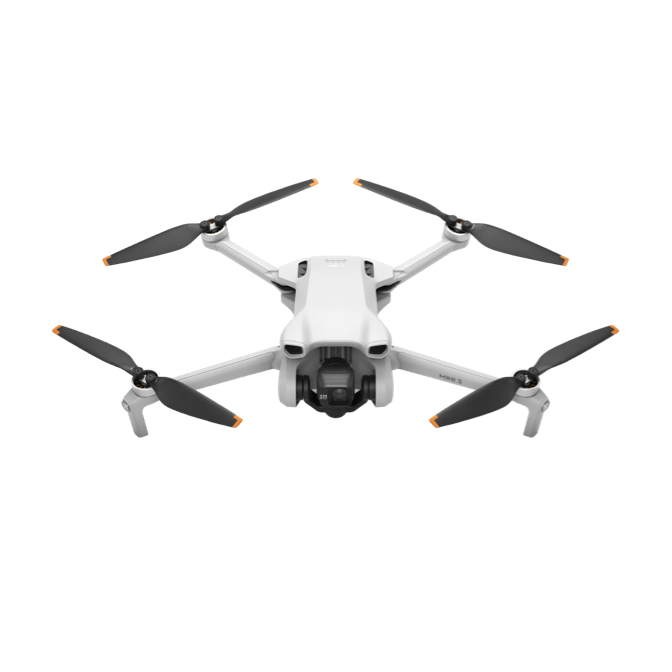
\includegraphics[width=\linewidth,height=4cm,keepaspectratio,trim=30 200 30 160,clip]{dji-mini-3.png}
\par\smallskip
{\small (a) DJI Mini~3}
\end{minipage}\hfill
\begin{minipage}[b]{0.48\textwidth}
\centering
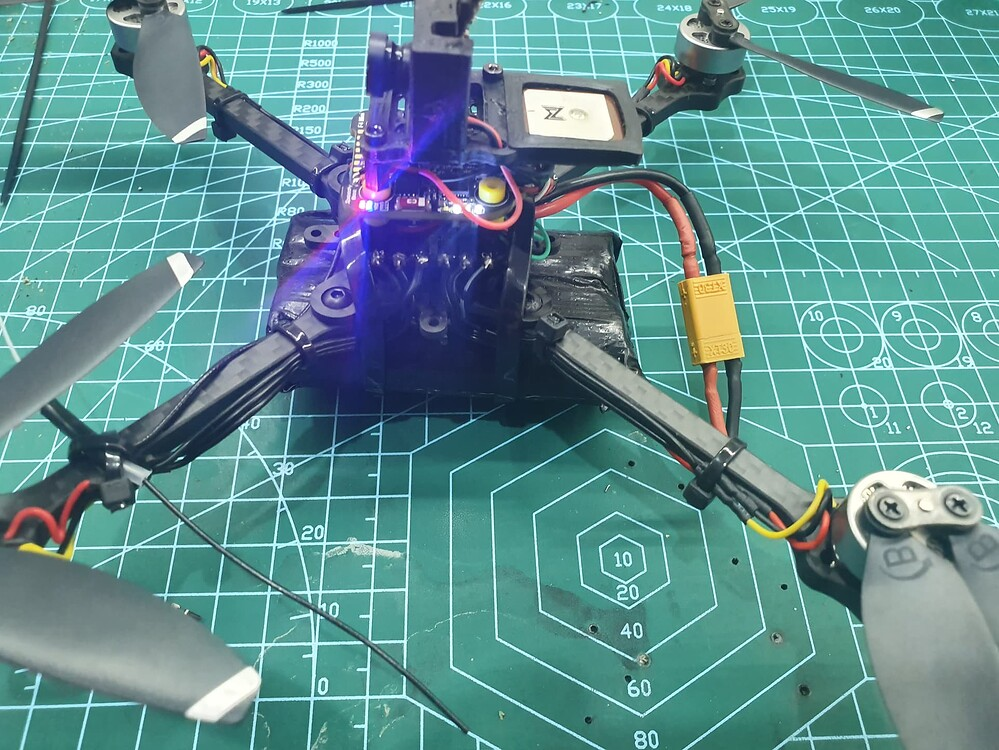
\includegraphics[width=\linewidth,height=4cm,keepaspectratio]{diy-250g-ardupilot.jpg}
\par\smallskip
{\small (b) Projeto DIY com ArduPilot}
\end{minipage}
\caption[DJI Mini 3 e projeto DIY para a classe sub-250 g]{(a) DJI Mini~3, imagem oficial da fabricante~\cite{mini3imagem}; (b) montagem do projeto \emph{250g endurance quadcopter}, fotografia publicada por geofrancis~\cite{diy250}. Imagens em escalas distintas; as margens vazias do painel (a) foram omitidas. A massa do DIY depende da configuração; a fotografia não constitui registro de pesagem.}
\label{fig:plataformas-sub250}
\end{figure}

\begin{table}[htbp]
\centering\small
\caption{Critérios para comparar o Mini~3 e uma montagem DIY na faixa sub-250~g. As informações de massa provêm da fabricante e do relato do construtor e se referem às configurações descritas no texto.}
\label{tab:sub250}
\begin{tabularx}{\textwidth}{@{}>{\raggedright\arraybackslash}p{2.8cm}YY@{}}
\toprule
Critério & DJI Mini~3 & DIY com ArduPilot \\
\midrule
Massa & 248~g na configuração padrão; cerca de 290~g com bateria Plus & Abaixo de 250~g sem GPS no relato; 260~g com GPS e suporte \\
Integração & Câmera, estabilizador e navegação integrados & Componentes, alimentação e montagem definidos pelo construtor \\
Acesso ao controle & Funções expostas pelo Mobile SDK compatível & Possibilidade de modificar o software de voo aberto \\
Sensores adicionais & Exigem verificar interfaces e massa final & Exigem verificar drivers, alimentação e massa final \\
Uso em enxames & Exige aplicação de coordenação e interfaces adequadas & Exige integrar localização, comunicação e coordenação \\
\bottomrule
\end{tabularx}
\end{table}

Para pesquisa sobre os controladores internos, uma montagem com pilha aberta permite intervir no software de voo. Essa liberdade acrescenta trabalho de montagem, calibração e manutenção. Para pesquisa centrada em aquisição de imagens ou aplicações nas interfaces disponíveis, a integração do Mini~3 pode reduzir etapas de construção. Para aproximar esses exemplos da função dos drones da floresta, seria necessário integrar localização, percepção de obstáculos, planejamento e comunicação entre agentes, respeitando a capacidade de processamento e de carga. A semelhança de porte não demonstra essa capacidade, e o suporte a um SDK não fornece, isoladamente, uma solução de enxame.
\FloatBarrier

\section{Competências técnicas e esforço de desenvolvimento}\label{sec:competencias}
Para os usos apresentados na Seção~\ref{sec:drones-pesquisa}, o esforço de desenvolvimento depende do acesso exigido ao hardware e ao software. A Tabela~\ref{tab:competencias} relaciona as tarefas às competências de integração. A distinção entre operar a aeronave, programar uma aplicação e modificar o firmware permite identificar quais conhecimentos o projeto exige.

\subsection{Operação, aplicações e alterações no firmware}
Na \emph{operação}, o trabalho envolve configurar a aeronave, interpretar modos de voo, verificar a localização e reconhecer condições que impedem executar a missão. O uso das funções prontas de uma plataforma comercial não exige, por si só, escrever programas ou projetar circuitos. Na montagem DIY, a preparação inclui conexões elétricas, instalação da pilha de voo e calibração. O guia de montagem Pixhawk exemplifica a ligação de alimentação, receptor, motores e sensores~\cite{px4montagem}.

No \emph{desenvolvimento de aplicações}, o programa recebe telemetria e envia comandos pelas interfaces disponíveis. Isso exige compreender a API, os sistemas de coordenadas, as unidades das mensagens, o tratamento de erros e o fluxo de execução. Em produtos DJI compatíveis, o trabalho depende do SDK e dos recursos expostos para o modelo~\cite{dji,djimobilesdk}. Em plataformas abertas, pode utilizar MAVLink ou interfaces ROS~2, conforme a configuração. Enviar referências por uma interface externa não exige necessariamente modificar o firmware da controladora~\cite{offboard}.

Na \emph{alteração do software embarcado}, a equipe passa a trabalhar com compilação, organização do código, depuração e verificação das mudanças. Alterar um controlador também exige compreender dinâmica, realimentação, estabilidade e limitações dos atuadores. A documentação de desenvolvimento e os diagramas do PX4 fornecem referências para esse nível de intervenção~\cite{px4desenvolvimento,controle}. Acesso ao código permite modificar o sistema, mas não demonstra que uma modificação preserve seu comportamento.

\FloatBarrier
\begin{table}[htbp]
\centering\small
\caption{Conhecimentos associados às tarefas de desenvolvimento em plataformas integradas e DIY.}
\label{tab:competencias}
\begin{tabularx}{\textwidth}{@{}>{\raggedright\arraybackslash}p{2.6cm}YY@{}}
\toprule
Área & Plataforma integrada, como DJI & DIY com pilha aberta \\
\midrule
Eletrônica & Identificar interfaces e limites elétricos ao conectar acessórios & Verificar tensão, corrente, polaridade, alimentação e conexões; soldar quando a montagem exigir \\
Programação & Desenvolver a aplicação no SDK compatível e tratar comandos, eventos e telemetria & Integrar a aplicação à pilha; modificar e compilar firmware quando necessário \\
Controle e estimação & Compreender modos de voo, referências e limitações das funções disponíveis & Calibrar sensores, ajustar parâmetros e analisar controladores ou estimadores conforme o objetivo \\
Comunicação & Compreender a ligação entre aplicação, controle remoto e aeronave & Configurar enlaces, portas e protocolos dos componentes escolhidos \\
Mecânica e energia & Verificar fixação, massa e compatibilidade dos acessórios & Selecionar estrutura, propulsão e bateria; verificar montagem, vibração e distribuição de massa \\
Diagnóstico & Interpretar telemetria e registros disponibilizados pelo produto & Correlacionar registros de voo com medições elétricas, sensores e versões do software \\
\bottomrule
\end{tabularx}
\end{table}

A base de eletrônica inclui tensão, corrente, potência, polaridade e leitura de diagramas de ligação. Na montagem e no diagnóstico, também envolve utilizar instrumentos, como multímetro, e reconhecer a diferença entre alimentação e sinais de comunicação. O uso de conectores prontos pode reduzir a soldagem; não elimina a necessidade de verificar compatibilidade elétrica~\cite{px4montagem}. Desenvolver uma aeronave com placas comerciais não exige necessariamente projetar uma placa eletrônica própria.

A base de programação inclui estruturas de dados, funções, tratamento de erros e leitura de documentação de interfaces. No desenvolvimento de sensores, acrescentam-se aquisição de dados, configuração de interfaces e sincronização dos registros. Para um novo algoritmo de controle, são necessárias a implementação das equações, a compreensão das frequências de atualização e a análise da resposta do veículo. Linguagens e ferramentas dependem da camada: a aplicação pode utilizar uma linguagem oferecida pela API, enquanto modificações no PX4 requerem seu ambiente de desenvolvimento~\cite{px4desenvolvimento}. Python, C++ e ROS~2 não constituem um conjunto obrigatório para toda plataforma.

\subsection{Esforço de integração conforme o objetivo}
As configurações da Tabela~\ref{tab:niveis} concentram dificuldades diferentes. Na simulação, predominam modelagem, programação e interpretação de resultados; a montagem eletrônica pode não participar da atividade. No laboratório com localização externa, acrescentam-se a calibração dessa infraestrutura e sua integração com os veículos. Na plataforma média aberta, a equipe assume a integração elétrica e mecânica, além da configuração e do diagnóstico da pilha de voo. Na plataforma micro com percepção embarcada, essas tarefas precisam respeitar limites mais estreitos de massa, energia e capacidade de processamento.

A complexidade também muda conforme o componente investigado. Um sensor próprio exige projeto ou integração do circuito, calibração e análise de incerteza. Um controlador exige modelagem dinâmica e análise das respostas de voo. Uma aplicação de inteligência artificial (IA) embarcada acrescenta preparação de dados, execução do modelo e verificação de latência e consumo. Uma carga útil exige verificar a influência de sua massa, fixação e alimentação. Essas tarefas podem ocorrer em uma única aeronave, tanto em plataforma integrada quanto em montagem própria.

A miniaturização acrescenta restrições às tarefas de integração, como mostra a comparação da Seção~\ref{sec:sub250}. Ela pode exigir componentes menores, revisão da alimentação e maior atenção à montagem e à dissipação térmica.

\subsection{Distribuição das competências na equipe}
Os compromissos entre acesso ao sistema e esforço de integração foram comparados na Seção~\ref{sec:dji-diy}. Para organizar o trabalho, essas diferenças precisam ser traduzidas em responsabilidades técnicas.

A escolha deve relacionar as tarefas às competências disponíveis na equipe. Para desenvolver missões nas interfaces de uma plataforma integrada, são centrais a programação da aplicação, a compreensão dos modos de voo e a análise da telemetria. Para pesquisar controladores em uma montagem aberta, acrescentam-se controle, desenvolvimento embarcado e diagnóstico elétrico. Para construir sensores, são centrais o projeto eletrônico, a aquisição e a calibração; para percepção baseada em IA, a preparação dos dados, a avaliação do modelo e sua integração ao processamento de bordo. Essas competências podem ser distribuídas entre pessoas; o planejamento precisa prever quem responde pela montagem, pelo software e pela análise dos dados.

\section{Requisitos da plataforma por área de pesquisa}\label{sec:areas-pesquisa}
A Seção~\ref{sec:drones-pesquisa} apresentou os usos de drones na pesquisa. Para selecionar uma aeronave, esses usos se traduzem em requisitos de interfaces, instrumentação, processamento e operação. Os critérios a seguir complementam a comparação entre plataformas integradas e abertas.

\subsection{Desenvolvimento de sensores e instrumentação}
Na construção de um sensor para uso embarcado, a plataforma precisa fornecer fixação, alimentação e uma interface para aquisição de dados. Também precisam ser considerados a faixa de medição, a calibração, o ruído, a taxa de amostragem e a sincronização com os registros do veículo. Vibração dos motores, aquecimento e interferência elétrica podem afetar a medição. A massa e a posição de montagem do instrumento, por sua vez, alteram a distribuição de massa da aeronave.

Um sensor destinado à navegação precisa fornecer informações no tempo exigido pelo estimador ou pelo controlador. Um instrumento de coleta ambiental pode registrar dados sem participar diretamente do controle de voo. Essa diferença determina se basta armazenar medições ou se é necessário integrar o dispositivo à pilha de navegação. O acesso a interfaces e computadores complementares, descrito na documentação PX4, participa dessa decisão~\cite{companion,px4montagem}. A precisão da trajetória e a qualidade da medição são propriedades distintas e precisam ser analisadas separadamente.

\subsection{Desenvolvimento de controle de voo e estimação}
Para modificar uma malha interna de controle, a plataforma precisa permitir acesso ao algoritmo, aos estados utilizados e aos comandos dos atuadores. Os diagramas do PX4, discutidos no Capítulo~\ref{cap:alg}, ajudam a identificar o ponto de intervenção~\cite{controle}. Os registros devem permitir relacionar referências e respostas do veículo, respeitando as frequências de atualização de cada módulo.

Uma montagem aberta de porte médio pode facilitar a instrumentação e as alterações de componentes. Isso não torna F450 ou X500 requisitos para pesquisa em controle: um microquadricóptero também pode atender ao estudo quando oferece as interfaces e os registros necessários. A escolha depende da dinâmica a investigar, da instrumentação e do acesso ao software. Erro de acompanhamento, atraso, saturação dos atuadores e sensibilidade a mudanças de massa são aspectos de análise; atingir o destino não caracteriza sozinho a resposta do controlador.

\subsection{Percepção, navegação autônoma e inteligência artificial}
Na integração de percepção e IA embarcada, a plataforma deve comportar câmera, processamento, alimentação e dissipação térmica. O dispositivo escolhido precisa executar o modelo no tempo disponível e fornecer seus resultados ao módulo de navegação. A decisão entre câmera inteligente, computador complementar e outro processador depende das interfaces, da memória e do consumo previstos.

O Swift, apresentado por Kaufmann et al., exemplifica essa integração em corrida autônoma: utilizou percepção visual e inercial e uma política de controle treinada por aprendizado por reforço, com sensores e processamento a bordo durante as provas~\cite{swift}. O resultado refere-se ao circuito e às condições avaliadas. Ele ilustra uma linha de pesquisa em autonomia de uma aeronave, distinta da coordenação cooperativa entre veículos.

Treinar um modelo e executá-lo a bordo são atividades diferentes. Além do tempo de cálculo e do consumo, a avaliação precisa considerar dados diferentes dos usados no treinamento e o efeito de atrasos ou falhas da percepção sobre os comandos de movimento. Uma estrutura maior pode facilitar a instalação inicial; a miniaturização exige reavaliar esses recursos.

\subsection{Cargas úteis e aquisição de dados}
Para integrar uma carga útil, ou \emph{payload}, devem ser especificados massa, fixação, campo de visão, alimentação e troca de comandos. A documentação PX4 apresenta interfaces para câmeras, cargas e instrumentação~\cite{px4payloads}. O equipamento precisa ser compatível tanto com a capacidade mecânica e elétrica da aeronave quanto com a aplicação de aquisição de dados.

F450, X500 e configurações de maior porte, incluindo hexacópteros, podem ser considerados quando o projeto exige espaço e capacidade de transportar equipamentos. O número de motores não determina sozinho a carga admissível ou a tolerância a falhas: essas propriedades dependem da propulsão, da estrutura, da alimentação e do controle. Uma plataforma integrada pode atender à coleta de dados quando o equipamento necessário e suas interfaces estão disponíveis. Uma montagem própria permite adaptar o arranjo físico, com o custo de integração correspondente.

Em mapeamento, inspeção ou monitoramento, a avaliação também envolve o produto obtido: cobertura, resolução, calibração e associação temporal e espacial das medições. A capacidade de decolar e percorrer uma rota não demonstra que os dados atendam à pergunta científica.

\subsection{Coordenação de múltiplas aeronaves}
A operação com vários veículos exige considerar repetição da montagem, disponibilidade de reposições, comunicação e espaço para operar o grupo. Os estudos do Capítulo~\ref{cap:casos} ilustram duas escolhas de integração: localização externa no Crazyswarm e percepção e planejamento embarcados no trabalho da floresta~\cite{crazyswarm,wildpaper}. Essas arquiteturas determinam quais recursos cada aeronave precisa transportar.

Plataformas compactas são relevantes quando a pergunta exige muitos agentes ou deslocamento por passagens estreitas. Aeronaves maiores também podem participar de sistemas cooperativos quando a tarefa exige carga ou instrumentação. Neste livro, os exemplos F450 e X500 representam principalmente possibilidades de integração para pesquisa individual; não são apresentados como configurações de referência dos enxames estudados. O porte e a quantidade de rotores descrevem a aeronave, enquanto o funcionamento como enxame depende de sua coordenação.


%======================================================================
\appendix

\chapter{Glossário de siglas}\label{ap:glossario}
\begin{table}[htbp]
\centering\small
\caption{Siglas utilizadas neste livro.}
\label{tab:glossario}
\begin{tabularx}{\textwidth}{@{}>{\raggedright\arraybackslash}p{2.5cm}Y@{}}
\toprule
Sigla & Significado \\
\midrule
API & \emph{Application Programming Interface}, interface de programação de aplicações \\
CBBA & \emph{Consensus-Based Bundle Algorithm}, algoritmo de alocação de tarefas \\
DIY & \emph{Do it yourself}, montagem feita pelo próprio pesquisador \\
EKF & \emph{Extended Kalman Filter}, filtro de Kalman estendido \\
ESC & \emph{Electronic Speed Controller}, controlador eletrônico de velocidade \\
GNSS/GPS & Navegação por satélite / Sistema de Posicionamento Global \\
IA & Inteligência artificial \\
IMU & \emph{Inertial Measurement Unit}, unidade de medição inercial \\
MAVLink & Protocolo de mensagens para veículos não tripulados \\
MPC & \emph{Model Predictive Control}, controle preditivo baseado em modelo \\
ORCA & \emph{Optimal Reciprocal Collision Avoidance} \\
PID & Controlador proporcional, integral e derivativo \\
ROS~2 & \emph{Robot Operating System}, infraestrutura de software para robótica \\
SDK & \emph{Software Development Kit}, kit de desenvolvimento de software \\
SGBA & \emph{Swarm Gradient Bug Algorithm} \\
SITL & \emph{Software-in-the-loop}, simulação com o \emph{software} de voo real \\
UWB & \emph{Ultra-wideband}, rádio de banda ultralarga \\
\bottomrule
\end{tabularx}
\end{table}

\chapter{Notação matemática}\label{ap:notacao}
A Tabela~\ref{tab:notacao} reúne os símbolos utilizados nas equações do texto. Os símbolos também são definidos nas seções em que aparecem.

\begin{table}[htbp]
\centering\small
\caption{Notação utilizada nas equações.}
\label{tab:notacao}
\begin{tabularx}{\textwidth}{@{}>{\raggedright\arraybackslash}p{2.4cm}Y@{}}
\toprule
Símbolo & Significado \\
\midrule
$x$, $u$ & Estado e comando (entrada de controle) de uma aeronave \\
$p_i$, $v_i$, $a_i$ & Posição, velocidade e aceleração do agente $i$ \\
$e$, $r$, $y$ & Erro, referência e medição \\
$K_P$, $K_I$, $K_D$ & Ganhos proporcional, integral e derivativo \\
$H$ & Horizonte de predição do MPC \\
$\ell$, $V_f$ & Custo por etapa e custo terminal do MPC \\
$\mathcal N_i$, $a_{ij}$ & Conjunto de vizinhos do agente $i$ e peso da interação com o vizinho $j$ \\
$z_i$ & Variável coordenada pelo consenso \\
\bottomrule
\end{tabularx}
\end{table}

%======================================================================
\backmatter
\clearpage
\phantomsection
\addcontentsline{toc}{chapter}{Referências}
\begin{thebibliography}{99}
\footnotesize
\setlength{\itemsep}{3pt}
\bibitem{survey} \emph{A Survey on Swarming With Micro Air Vehicles: Fundamental Challenges and Constraints}. Frontiers in Robotics and AI, 2020. \url{https://doi.org/10.3389/frobt.2020.00018}.
\bibitem{crazyswarm} Preiss, J. A.; Hönig, W.; Sukhatme, G. S.; Ayanian, N. \emph{Crazyswarm: A Large Nano-Quadcopter Swarm}. ICRA, 2017. \url{https://whoenig.github.io/publications/2017_ICRA_Preiss_Hoenig.pdf}.
\bibitem{wildcode} ZJU FAST Lab. \emph{EGO-Planner-v2: código associado a Swarm of micro flying robots in the wild}. \url{https://github.com/ZJU-FAST-Lab/EGO-Planner-v2}.
\bibitem{wildpaper} Zhou, X. et al. \emph{Swarm of micro flying robots in the wild}. Science Robotics, v.~7, eabm5954, 2022. \url{https://doi.org/10.1126/scirobotics.abm5954}. Cópia disponibilizada pelo autor: \url{https://zhepeiwang.github.io/pubs/sr_2022_swarm.pdf}.
\bibitem{ekf} PX4. \emph{Using PX4's Navigation Filter (EKF2)}. Documentação técnica (versão \emph{main}). \url{https://docs.px4.io/main/en/advanced_config/tuning_the_ecl_ekf}.
\bibitem{controle} PX4. \emph{Controller Diagrams}. Documentação técnica (versão \emph{main}). \url{https://docs.px4.io/main/en/flight_stack/controller_diagrams}.
\bibitem{dmpc} Gräfe, A.; Eickhoff, J.; Zimmerling, M.; Trimpe, S. \emph{DMPC-Swarm: Distributed Model Predictive Control on Nano UAV Swarms}. Autonomous Robots, v. 49, artigo 28, 2025. \url{https://doi.org/10.1007/s10514-025-10211-w}. Repositório: \url{https://github.com/Data-Science-in-Mechanical-Engineering/DMPC-Swarm}.
\bibitem{boids} Reynolds, C. W. Flocks, herds and schools: a distributed behavioral model. \emph{ACM SIGGRAPH Computer Graphics}, v. 21, n. 4, p. 25--34, 1987. \url{https://doi.org/10.1145/37402.37406}. Página do autor: \url{https://www.red3d.com/cwr/boids/}.
\bibitem{orca} van den Berg, J.; Guy, S. J.; Lin, M.; Manocha, D. Reciprocal n-body collision avoidance. In: \emph{Robotics Research} (ISRR 2009), Springer, 2011, p. 3--19. \url{https://doi.org/10.1007/978-3-642-19457-3_1}. Página dos autores: \url{https://gamma-web.iacs.umd.edu/ORCA/}.
\bibitem{ego} Zhou, X.; Zhu, J.; Zhou, H.; Xu, C.; Gao, F. \emph{EGO-Swarm: A Fully Autonomous and Decentralized Quadrotor Swarm System in Cluttered Environments}. ICRA, 2021. \url{https://arxiv.org/abs/2011.04183}.
\bibitem{consenso} Olfati-Saber, R.; Fax, J. A.; Murray, R. M. Consensus and cooperation in networked multi-agent systems. \emph{Proceedings of the IEEE}, v. 95, n. 1, p. 215--233, 2007. \url{https://doi.org/10.1109/JPROC.2006.887293}.
\bibitem{cbba} Choi, H.-L.; Brunet, L.; How, J. P. Consensus-based decentralized auctions for robust task allocation. \emph{IEEE Transactions on Robotics}, v. 25, n. 4, p. 912--926, 2009. \url{https://doi.org/10.1109/TRO.2009.2022423}.
\bibitem{uwbvio} Xu, H.; Wang, L.; Zhang, Y.; Qiu, K.; Shen, S. Decentralized visual-inertial-UWB fusion for relative state estimation of aerial swarm. \emph{ICRA}, 2020. \url{https://arxiv.org/abs/2003.05138}.
\bibitem{companion} PX4. \emph{Companion Computers}. Documentação técnica (versão \emph{main}). \url{https://docs.px4.io/main/en/companion_computer/}.
\bibitem{offboard} PX4. \emph{Offboard Mode}. Documentação técnica (versão \emph{main}). \url{https://docs.px4.io/main/en/flight_modes/offboard}.
\bibitem{config} PX4. \emph{Multicopter Configuration}. Documentação técnica (versão \emph{main}). \url{https://docs.px4.io/main/en/config_mc/}.
\bibitem{px4sim} PX4. \emph{Simulation}. Documentação técnica (versão \emph{main}). \url{https://docs.px4.io/main/en/simulation/}.
\bibitem{ardusitl} ArduPilot. \emph{SITL Simulator (Software in the Loop)}. Documentação de desenvolvimento. \url{https://ardupilot.org/dev/docs/sitl-simulator-software-in-the-loop.html}.
\bibitem{gazebo} Open Robotics. \emph{Gazebo}. \url{https://gazebosim.org/}.
\bibitem{airsim} Shah, S.; Dey, D.; Lovett, C.; Kapoor, A. AirSim: high-fidelity visual and physical simulation for autonomous vehicles. In: \emph{Field and Service Robotics}, Springer, 2018. \url{https://doi.org/10.1007/978-3-319-67361-5_40}.
\bibitem{bitcraze} Bitcraze. \emph{Crazyflie 2.1 Brushless}. Documentação da plataforma e interfaces. \url{https://www.bitcraze.io/products/crazyflie-2-1-brushless/}.
\bibitem{dji} DJI. \emph{Onboard SDK}. Recursos e produtos compatíveis. \url{https://developer.dji.com/onboard-sdk/}.
\bibitem{m300imagem} DJI. \emph{Support for Matrice 300 RTK}. Imagem e documentação oficial da plataforma. \url{https://www.dji.com/support/product/matrice-300}.
\bibitem{x500imagem} PX4. \emph{Holybro X500 V2 + Pixhawk 6C (PX4 Dev Kit)}. Guia de montagem e fotografia da plataforma. \url{https://docs.px4.io/main/en/frames_multicopter/holybro_x500v2_pixhawk6c}.
\bibitem{mcguire} McGuire, K. \emph{Autonomous swarms of tiny flying robots}. Tese de doutorado, TU Delft, 2019. Capítulo sobre Swarm Gradient Bug Algorithm. \url{https://research.tudelft.nl/files/62178603/knmcguire_dissertation_combined_final.pdf}.
\bibitem{dados} MAVLab, TU Delft. \emph{Minimal navigation solution for a swarm of tiny flying robots to explore an unknown environment}. Página de dados do artigo, 2019. \url{https://mavlab.tudelft.nl/minimal-navigation-solution-for-a-swarm-of-tiny-flying-robots-to-explore-an-unknown-environment/}. Artigo associado: \url{https://doi.org/10.1126/scirobotics.aaw9710}.
\bibitem{swarmlab} Soria, E.; Schiano, F.; Floreano, D. \emph{SwarmLab: a Matlab Drone Swarm Simulator}. IROS, 2020, p. 8005--8011. \url{https://doi.org/10.1109/IROS45743.2020.9340854}. Preprint: \url{https://arxiv.org/abs/2005.02769}.
\bibitem{swarmrepo} LIS--EPFL. \emph{SwarmLab}. Repositório do simulador. \url{https://github.com/lis-epfl/swarmlab}.
\bibitem{qgc} QGroundControl. \emph{QGroundControl: estação de solo para MAVLink}. \url{http://qgroundcontrol.com/}.
\bibitem{crazyswarm2} IMRCLab. \emph{Crazyswarm2}. \url{https://imrclab.github.io/crazyswarm2/}.
\bibitem{px4gazebo} PX4. \emph{Gazebo Simulation}. Documentação técnica. \url{https://docs.px4.io/main/en/sim_gazebo_gz/}.
\bibitem{gazebomundos} PX4. \emph{Gazebo Worlds}. Cenários e imagens da simulação. \url{https://docs.px4.io/main/en/sim_gazebo_gz/worlds}.
\bibitem{qgcplanejamento} QGroundControl. \emph{Plan View}. Documentação e imagem da interface de planejamento. \href{https://docs.qgroundcontrol.com/master/en/qgc-user-guide/plan_view/plan_view.html}{Acesso à documentação}.
\bibitem{jiahaoswarm} Jiahao. \emph{Swarm Simulation}. Descrição do projeto e demonstrações em Gazebo e AirSim, 2018. \url{https://www.jiahaoz.com/swarm-simulation}.
\bibitem{mini3spec} DJI. \emph{DJI Mini 3: Specs}. Massa e especificações da plataforma. \url{https://www.dji.com/mini-3/specs}.
\bibitem{mini3imagem} DJI. \emph{Support for DJI Mini 3}. Imagem e documentação oficial. \url{https://www.dji.com/support/product/mini-3}.
\bibitem{djimobilesdk} DJI. \emph{Mobile SDK}. Produtos compatíveis e documentação de desenvolvimento. \url{https://developer.dji.com/mobile-sdk/}.
\bibitem{diy250} geofrancis. \emph{250g endurance quadcopter}. Relato de construção e fotografias, ArduPilot Discourse, 2024. \url{https://discuss.ardupilot.org/t/250g-endurance-quadcopter/114365}.
\bibitem{px4montagem} PX4. \emph{Pixhawk Wiring Quick Start}. Ligações e integração dos componentes. \url{https://docs.px4.io/main/en/assembly/quick_start_pixhawk}.
\bibitem{px4desenvolvimento} PX4. \emph{PX4 Development}. Documentação de desenvolvimento. \url{https://docs.px4.io/main/en/development/development}.
\bibitem{px4payloads} PX4. \emph{Payloads and Cameras}. Interfaces de cargas úteis e instrumentação. \url{https://docs.px4.io/main/en/payloads/index}.
\bibitem{swift} Kaufmann, E. et al. \emph{Champion-level drone racing using deep reinforcement learning}. Nature, v.~620, p.~982--987, 2023. \url{https://doi.org/10.1038/s41586-023-06419-4}. Cópia dos autores: \url{https://rpg.ifi.uzh.ch/docs/Nature23_Kaufmann.pdf}.
\end{thebibliography}
\end{document}
